\documentclass{InsightBook}

% \usepackage{graphicx}
\usepackage{cite}
\usepackage{subfigure}
\usepackage{graphicx}
\usepackage[font=sf]{caption}
\usepackage{enumerate}
\usepackage{fancyhdr}
% \usepackage{fncychap}
% \usepackage{float}
\usepackage{floatflt}
\usepackage{amsmath}
\usepackage[tight]{units}
\usepackage{url}
\usepackage{xspace}
\usepackage[pdftex,bookmarksopen=true,bookmarksopenlevel=10,pdfstartview=Fit,bookmarks=true,colorlinks=true,linkcolor=blue,urlcolor=blue,citecolor=blue,pdfauthor={Daniel J. Blezek and James V. Miller},pdftitle={Dart Manual}]{hyperref}


\newcommand{\answermark}{$\triangleright$ }
\newcommand{\xmltag}[1]{\texttt{<#1>}}

% Use to markup file and directory names
\newcommand{\filename}[1]{\texttt{#1}}

% This declares a set of common abbreviations (e.g., i.e.,
% etc.). These commands should be used instead of explicitly doing it
% yourself to get better typeset results. For example, ``\emph{e.g.}
% something'' would yield a sentence ending space between the ``.''
% and ``s'', which is not correct. The correct way is ``\emph{e.g.}\
% something''; this inserts a normal interword space. The macro
% ``\eg'' will take care of this automatically. The macros below will
% also make sure that at the end of a sentence, there won't be two
% periods. \Ie, ``apples, bananas, \etc.'' will not have two periods
% at the end, but ``(apples, bananas, \etc)'' will have a period
% before the closing paranthesis.
%
% (The code below taken from cvpr.sty, by Paolo.Ienne@di.epfl.ch 
% and awf@acm.org.)
%
\makeatletter
\DeclareRobustCommand\onedot{\futurelet\@let@token\@onedot}
\def\@onedot{\ifx\@let@token.\else.\xspace\fi}
\def\eg{\emph{e.g}\onedot} \def\Eg{\emph{E.g}\onedot}
\def\ie{\emph{i.e}\onedot} \def\Ie{\emph{I.e}\onedot}
\def\cf{\emph{c.f}\onedot} \def\Cf{\emph{C.f}\onedot}
\def\etc{\emph{etc}\onedot}
\def\vs{\emph{vs}\onedot}
\def\wrt{w.r.t\onedot}
\def\dof{d.o.f\onedot}
\def\etal{\emph{et al}\onedot}
\makeatother


\begin{document}
\title{Dart: Testing, Reports and Dashboards}
\author{Daniel J. Blezek \\
James V. Miller}
\maketitle


%----------------------------------------------------------------------
\chapter*{Acknowledgments}
\thispagestyle{empty}
This product includes software developed by the Apache Software Foundation (\url{http://www.apache.org/}).

This product includes software developed by the Visigoth Software Society (\url{http://www.visigoths.org/}).

This work funded in part by the National Library of Medicine of the National Institutes of Health as a component of the Insight Segmentation and Registration Toolkit (\url{http://www.itk.org/}), contract number N01-LM-9-3531.

This work is part of the National Alliance for Medical Image
Computing (NA-MIC), funded by the National Institutes of Health
through the NIH Roadmap for Medical Research, Grant U54 EB005149.
Information on the National Centers for Biomedical Computing
can be obtained from \url{http://nihroadmap.nih.gov/bioinformatics}.

%----------------------------------------------------------------------
\chapter*{License}
\thispagestyle{empty}
\begin{verbatim}
Copyright (c) 2004-2005, The Insight Consortium
All rights reserved.

Redistribution and use in source and binary forms, with or without
modification, are permitted provided that the following conditions are
met:

* Redistributions of source code must retain the above copyright
notice, this list of conditions and the following disclaimer.
* Redistributions in binary form must reproduce the above copyright
notice, this list of conditions and the following disclaimer in the
documentation and/or other materials provided with the distribution.
* Neither the name of the Insight Consortium nor the names of its
contributors may be used to endorse or promote products derived from
this software without specific prior written permission.

THIS SOFTWARE IS PROVIDED BY THE COPYRIGHT HOLDERS AND CONTRIBUTORS
"AS IS" AND ANY EXPRESS OR IMPLIED WARRANTIES, INCLUDING, BUT NOT
LIMITED TO, THE IMPLIED WARRANTIES OF MERCHANTABILITY AND FITNESS FOR
A PARTICULAR PURPOSE ARE DISCLAIMED. IN NO EVENT SHALL THE COPYRIGHT
OWNER OR CONTRIBUTORS BE LIABLE FOR ANY DIRECT, INDIRECT, INCIDENTAL,
SPECIAL, EXEMPLARY, OR CONSEQUENTIAL DAMAGES (INCLUDING, BUT NOT
LIMITED TO, PROCUREMENT OF SUBSTITUTE GOODS OR SERVICES; LOSS OF USE,
DATA, OR PROFITS; OR BUSINESS INTERRUPTION) HOWEVER CAUSED AND ON ANY
THEORY OF LIABILITY, WHETHER IN CONTRACT, STRICT LIABILITY, OR TORT
(INCLUDING NEGLIGENCE OR OTHERWISE) ARISING IN ANY WAY OUT OF THE USE
OF THIS SOFTWARE, EVEN IF ADVISED OF THE POSSIBILITY OF SUCH DAMAGE.
\end{verbatim}

% Put the table on contents after the license
%
%
%
\tableofcontents
\setcounter{tocdepth}{10}


%----------------------------------------------------------------------
\chapter{Introduction}

\section{Dart Statement of Purpose}
\begin{quote}
\emph{Dart shall aggregate data across many independent distributed
build and test hosts, summarizing the software quality aspects of the project
in a concise and informative fashion cross-sectionally and longitudinally.}
\end{quote}

\section{History of Dart}
In 1997, General Electric added a new quality initiative, called \emph{Six Sigma}.  As part of Six Sigma training, each employee had to complete a number of quality projects.  At GE Research, we focused a collection of our quality projects on the development of one of our software toolkits, the Visualization Toolkit or VTK (\url{http://www.vtk.org/}).  At the end of the first round of training, we had 14 different quality assurance processes applied to dynamic memory analysis, test code coverage, coding style, etc. In a second round of training, we integrated these original 14 projects into an automated system that collected their outputs and integrated them into an online dashboard. This system was a collection of \texttt{tcsh}, \texttt{awk}, \texttt{sed} and \texttt{cron} scripts, cobbled together into a quality assurance system.

In 1999, the National Library of Medicine commissioned the development of an open source, cross platform project called the Insight Segmentation and Registration Toolkit, ITK (\url{http://www.itk.org/}).  As part of GE Research's contribution to the ITK effort, GE Research developed the first version of Dart.  Dart's goals were
\begin{enumerate}
\item Remove the dependence on \texttt{tcsh}, \texttt{awk}, \texttt{sed} and \texttt{cron} scripts to perform a build and test sequence
\item Allow testing machines from around the world to submit test results to a Dart server
\item Separate the data from its presentation
\item Apply the Dart testing system to a variety of project (ITK, VTK, VXL)
\item Make the testing system itself open source
\end{enumerate}
The original Dart used \texttt{TCL} to orchestrate a build/test sequence on a client machine and construct an XML representation of the build/test results.  The XML files were sent to a staging area on a Dart server using \texttt{ftp} and a \texttt{cgi-bin} script moved the XML data to the Dart server web page. A \texttt{cron} job periodically rolled up a Dashboard, using XSLT to convert the XML files to static HTML.  Later, Kitware Inc. developed a second Dart client called CTest.  CTest simplified the build/test process for the client machines and removed the client's dependency on \texttt{TCL}.

Dart met its original design goals and was successfully applied to many software projects. Dart clients were easy to use and allowed for testing machines to be distributed around the world.  The Dart server allowed anyone to view the results of a test sequence and monitor the software development process.  Dart allowed a cross-platform system to be tested in multiple configurations.

The server side of Dart, however, was still difficult to maintain.  The Dart server needed a web server, cgi-bin, \texttt{Perl}, an \texttt{ftp} server, \texttt{TCL}, \texttt{cron}, and \texttt{java} (for XSLT). Dart required considerable storage and computational resources.  The XML files needed considerable storage and it could take 20 minutes to convert XML files into static web pages. 

In 2004, NIH sponsored the National Alliance of Medical Image Computing, NA-MIC (\url{http://www.na-mic.org/}) as part of NIH Roadmap for Medical Research, Grant U54 EB005149.  GE Research is developing the next generation of Dart as part of NA-MIC.  The goals remain broadly the same, however, two new goals have been identified
\begin{enumerate}
\item Simplify the Dart server setup and maintenance
\item Allow for longitudinal or temporal analysis of test results
\end{enumerate}

To this end, we introduce the new version of Dart.  We affectionately refer to the previous version of Dart as \emph{Dart Classic}.   The new Dart still accepts build/test results in the \emph{Dart Classic} format.  Dart has been completely rewritten in Java.  It uses an embedded web server and servlet engine (Jetty) and an embedded database (Derby).  XML-RPC is used to transmit build/test results to the Dart server.  Dart is distributed as two jar files.  The first jar file, DartServer.jar, contains everything to create and run a Dart server managing serveral Dart projects.  The second jar file, DartClient.jar, is a small utility to shutdown a server, refresh its resources, query its status, and can be used as an XML-RPC messenger.


\section{To Do}
\begin{itemize}
\item Calendar for easy day navigation
\item Fix display of gcov results, not currently indented correctly
\item Use Javascript column sorting, rather than server side sorting
\item HTAccess support 
\begin{verbatim}
 <Directory "/">
      <limit GET POST>
      Order deny,allow
      deny from all
      allow from 127.0.0.1
      </Limit>
 </Directory>
\end{verbatim}
\item SSL support
\end{itemize}

%----------------------------------------------------------------------
\chapter{Tutorial}

\section{Quick Start}
\label{Section:QuickStart}

If you are building Dart from source, please refer to
Section~\ref{Section:Development} to build the jar files, then return
to this Section.  If you've downloaded the jar files, you may begin
here.  The distributions are built using JDK 1.4.  For users upgrading
from an earlier version of Dart, please see Sections~\ref{Section:UpgradeServer}-\ref{Section:UpgradePre0.4}.

Dart contains two jar files:
\begin{description}
\item[DartServer.jar] Complete Dart server with http server, servlet engine, and backend database.
\item[DartClient.jar] Small client to communicate with the Dart server.  DartClient.jar can be used to shutdown the server, instruct the server to refresh/restore its resources (icons, templates, styles) from the DartServer.jar file, query the status of the Dart server, and transmit XML files to the Dart server.
\end{description}

Here are the steps to create a new Dart server, create a project on the Dart server, and start and stop the Dart server:
\begin{enumerate}
    \item Create the Server directory and configuration\\
    \begin{verbatim}
java -jar DartServer.jar --createserver TestServer
    \end{verbatim}
    The \texttt{--createserver} flag creates a new Server directory and an default configuration file Server.xml.
    \item Initialize the server\\
    \begin{verbatim}
java -jar DartServer.jar --initializeserver TestServer
    \end{verbatim}
    Initializes the Server database.
    \item Create the project\\
    \begin{verbatim}
java -jar DartServer.jar  --create TestProject
    \end{verbatim}
    The \texttt{--create} flag requires a directory name argument.
    Dart will create this directory for the Project
    (\texttt{TestProject} in this example).

    \item Configure the Project
    By default, a reasonable settings file is found in
    \texttt{TestProject/Project.xml}.  If desired, this file may be
    edited to change the projects settings (see
    Section~\ref{Section:Settings}).  Now is a good time to do this.

    \item \label{quickstart:startprojectfirsttime} Start the project for the first time\\
    \begin{verbatim}
java -jar DartServer.jar \
              --initialize --refresh --refreshServer TestServer TestProject
    \end{verbatim}
    The \texttt{--initialize} flag instructs the server to create the
    database tables that Dart requires for the project, while \texttt{--refresh}
    copies the project resources into the TestProject directory.
    TestServer is the name of the Dart Server, while any projects to
    be started can be configured in TestServer/Server.xml and are
    overridden by the commandline arguments. Note that \textbackslash\
    indicates line continuation; that is, the code above should be
    typed on one line.  The \texttt{--refreshServer} puts some server
    specific files in the correct locations in the Server directory.
    \item View the dashboard.  Point your browser to
          \texttt{http://localhost:8081/TestProject/Dashboard/} to
          view the (empty) Dashboard.         
    \item Shutting down the server
    \begin{verbatim}
java -jar DartClient.jar -q TestProject
    \end{verbatim}
    To shutdown down the server, you need to send a message to the running server.  The DartClient.jar file is a small Dart client that can be used to shutdown the server (or query its status or refresh its resources).
    \item Restarting the server  
    \begin{verbatim}
java -jar DartServer.jar TestServer TestProject
    \end{verbatim}
    Once the project has been initialized in step \ref{quickstart:startprojectfirsttime}, the \texttt{--initialize} option is no longer needed when starting the project. The \texttt{--refresh} and \texttt{--refreshServer} could still be used if project or server resources (icons, template, styles) needed to be updated from the DartServer.jar.
\end{enumerate}
The project \texttt{TestProject} is now up and running accepting
XML-RPC submissions and serving HTML pages on
port \texttt{8081}.  The ports and other configurations are covered in
Section~\ref{Section:ServerSetup}.

\section{Web configuration}
\label{Section:WebConfiguration}
Once the Project is configured and the server is running, you should log into 
the Dart web application and configure the \texttt{admin} User.  Point a browser at 
\url{http://localhost:8081/TestProject/Dashboard/} (Figure \ref{fig:FirstDartPage}) and click on the \texttt{login or create account} link at the top of the page. Log in as the default Dart administrator (Figure \ref{fig:DartAdminLogin}) using 
\begin{description}
\item[Email:] admin
\item[Password:] password
\end{description}
Once you are logged into the Dart web application, you can modify the default password for the \texttt{admin} user (Figure \ref{fig:AdminUserPage}).

\begin{figure}[htb]
	\centering
		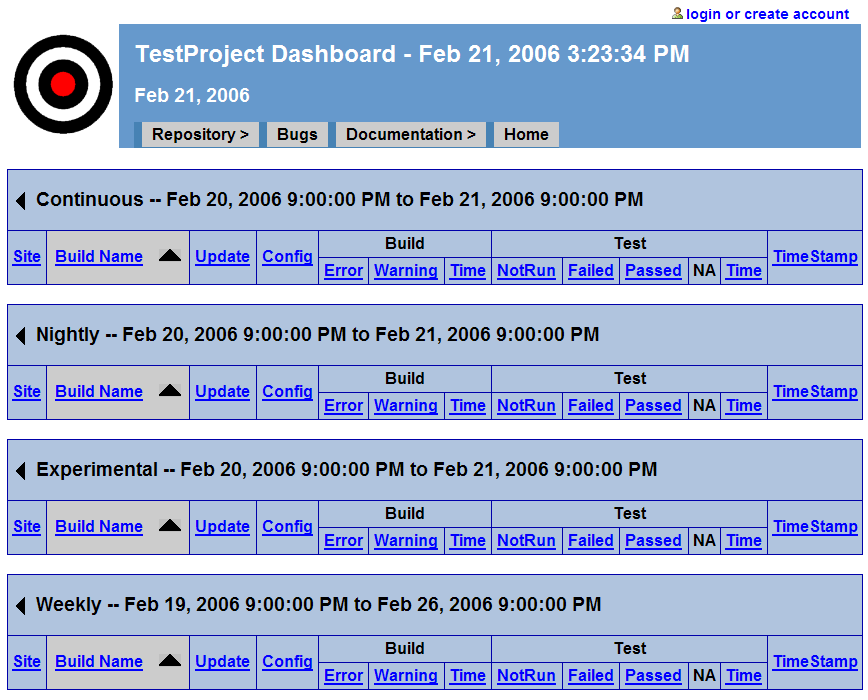
\includegraphics[width=4in]{FirstDartPage}
	\caption{Dart Dashboard}
	\label{fig:FirstDartPage}
\end{figure}

\begin{figure}[htb]
	\centering
		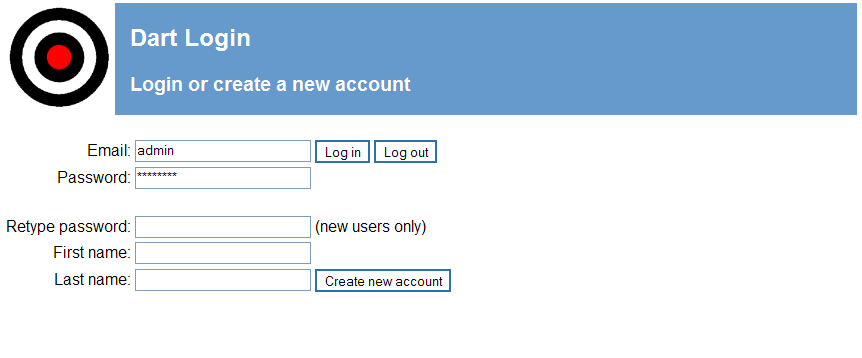
\includegraphics[width=4in]{DartAdminLogin}
	\caption{Logging in as the administrator}
	\label{fig:DartAdminLogin}
\end{figure}

\begin{figure}[htb]
	\centering
		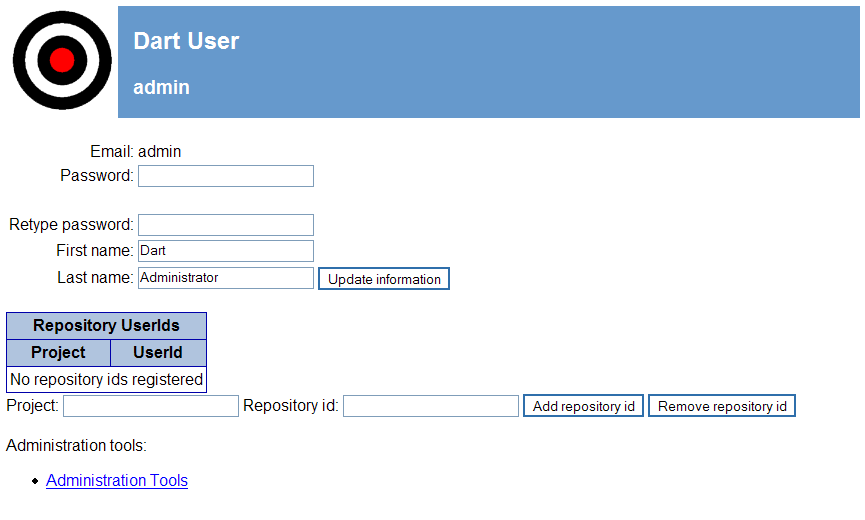
\includegraphics[width=4in]{AdminUserPage}
	\caption{Administrators User page}
	\label{fig:AdminUserPage}
\end{figure}


\section{Submission}
Dart ships with a utility called DartClient to submit results to the
server.  The basic use is:
\begin{verbatim}
java -jar DartClient.jar TestProject Results.xml
\end{verbatim}

This submits Results.xml to the \texttt{TestProject} Project on the
Server running on \texttt{localhost}.  Submission is only a copy, and
does not provide feedback on the XML validity.

DartClient also provides other options:
\begin{verbatim}
# java -jar DartClient.jar --help
0 [main] INFO dart.DartClient  - Starting DartClient
usage: DartClient [options] Project <foox.xml> <foo2.xml> ... <fooN.xml>
 -g,--getstatus   Get Server status
 -h,--help        Print help message
 -p,--port        XML-RPC Port to connect to, 8081 is default
 -q,--shutdown    Shutdown the Server
 -r,--refresh     Refresh Project resources
 -s,--server      Server to connect to, localhost is default
\end{verbatim}

To connect through a proxy or firewall use:
\begin{verbatim}
java -Dhttp.proxyPort=8080 -Dhttp.proxyHost=proxyhost.mydomain.org \
     -jar DartClient.jar --help
\end{verbatim}
with \texttt{http.proxyPort} and \texttt{http.proxyHost} replaced by
your proxy port and server.

\section{Software Installation}
To be completed.

\chapter{User Guide}
\label{Section:Users}
\section{Dart Users}

The Dart web application supports users and roles.  At the top of each Dart page is a link that allows one to \emph{login or create account} (Figure \ref{fig:FirstDartPage}).  Dart User accounts are shared amongst all projects on the Dart server. Currently, Dart User accounts are used by the Dart system to notify users of events. Future versions of Dart will allow Users more customization options: setting plot durations, storing queries, etc.

One event in the Dart system that may notify Users is a submission to the server that contains build errors.  The authors of the new code in that submission can be notified via email that their contribution or modification of the source code produces errors on a particular platform. The Dart server uses Dart User accounts to map from source code repository userids to email addresses for notifications.

\begin{figure}
	\centering
		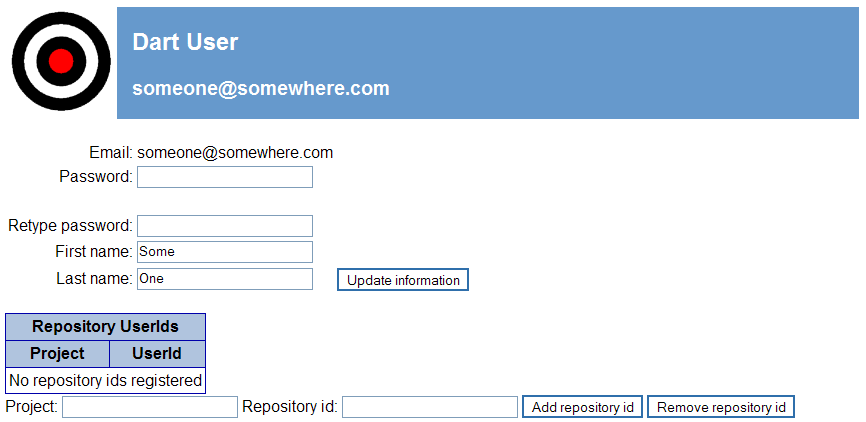
\includegraphics[width=4in]{DartUserPage}
	\caption{User page}
	\label{fig:DartUserPage}
\end{figure}


\begin{figure}
	\centering
		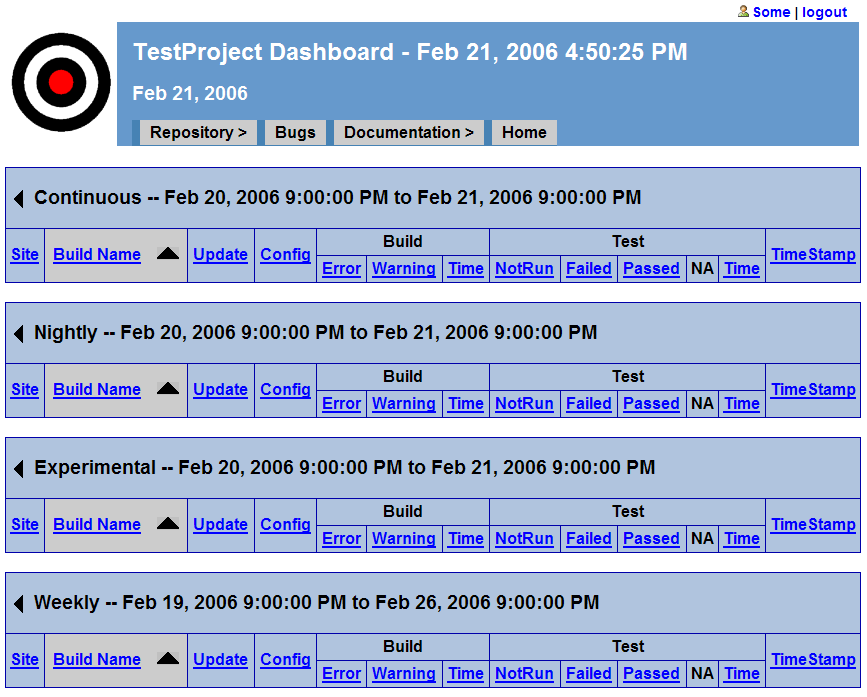
\includegraphics[width=4in]{DartPageWithUserLoggedIn}
	\caption{You can return to your Dart User page by clicking on your name at the top a Dart page.}
	\label{fig:DartPageWithUserLoggedIn}
\end{figure}


When you log into the Dart web application, you are taken to a page with your User properties (Figure \ref{fig:DartUserPage}). If you have already browsed off this page, you can return to this page at anytime by clicking on your name shown at the top of each Dart page (Figure \ref{fig:DartPageWithUserLoggedIn}.  The User property page has a table called \texttt{Repository Userids}.  The text entry controls at the bottom of this table allow the user to specify their source code repository userids for each Project hosted on the Dart server.  Figure \ref{fig:DartUserEnteringRepositoryId} shows how to associate the source code repository userid of \texttt{someone} to this User on the Project \texttt{TestProject}.  Figure \ref{fig:DartUserWithRepositoryId} shows the results of this association.  Multiple source code repository userids can be associated with a Dart User for one Project or for multiple Projects.


\begin{figure}
	\centering
		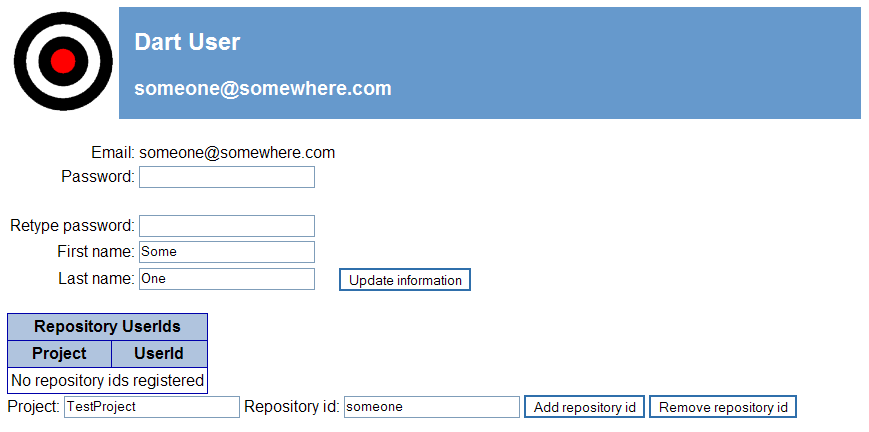
\includegraphics[width=4in]{DartUserEnteringRepositoryId}
	\caption{Enter source code repository userid associations for each Dart Project.}
	\label{fig:DartUserEnteringRepositoryId}
\end{figure}

\begin{figure}
	\centering
		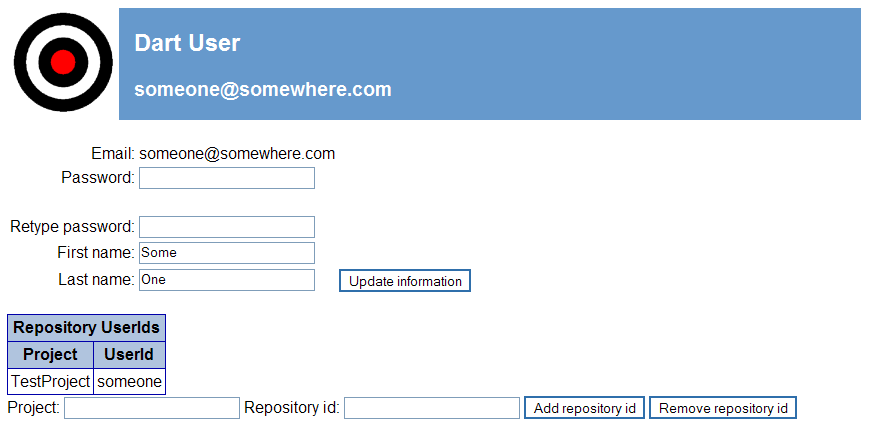
\includegraphics[width=4in]{DartUserWithRepositoryId}
	\caption{Dart User with a source code repository userid association.}
	\label{fig:DartUserWithRepositoryId}
\end{figure}

\section{Dart Navigation}

\section{Dashboard customization}

It is possible for the user to customize the information display on the Dashboard. Currently, url parameters can be used to control what tracks are displayed.  Adding url parameters like \texttt{showtrack=Nightly} will restrict the Dashboard display to just the Nightly track.  Using url parameters \texttt{showtrack=Nightly\&showtrack=Coverage} will display just the Nightly track and the Coverage track.

Future versions of Dart will allow these customizations to be stored as User specific queries.


\section{RSS Feeds}
\begin{floatingfigure}[l]{16pt}

\includegraphics[width=16pt]{feed-icon32x32.png}
\end{floatingfigure}
The Dashboard for any given Project can be monitored for new submissions by watching the provided RSS feed. In the title block on the Dashboard page, the RSS icon displayed is a hyperlink to the Project's RSS page.  You can copy the link associated with this image and paste the link into your RSS reader.

If use the FireFox browser, the RSS icon will appear in the address bar, indicating a RSS feed is available. You can add the RSS feed to your \emph{Live Bookmarks} by clicking on the icon.


\chapter{Dart Server and Project Administration Guide}

\section{Client Configuration}
\label{Section:ClientConfiguration}

\begin{figure}
	\centering
		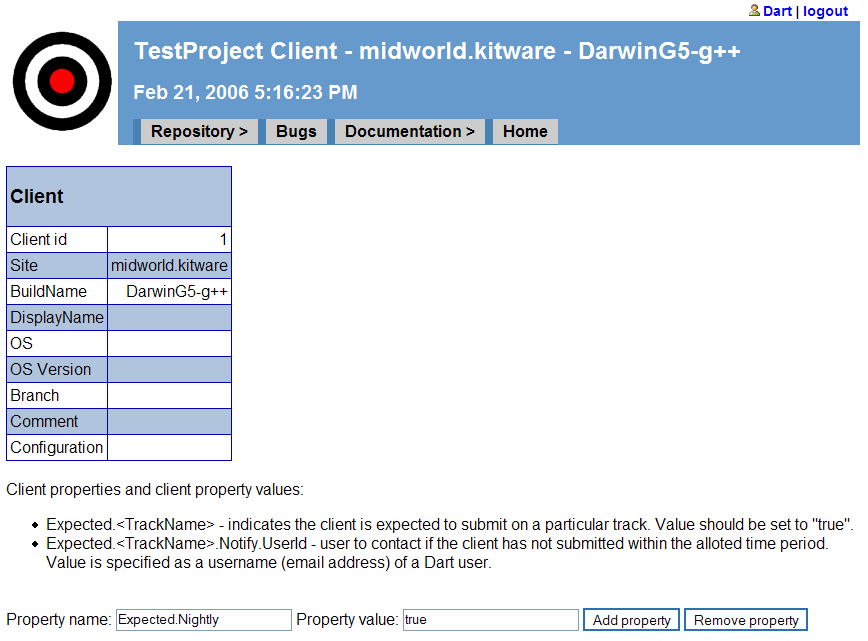
\includegraphics[width=4in]{ClientEnteringExpected}
	\caption{Designating a client as an expected submission requires a client property of \texttt{Expected.<TrackName>} with a value of \texttt{true}.}
	\label{fig:ClientEnteringExpected}
\end{figure}

\begin{figure}
	\centering
		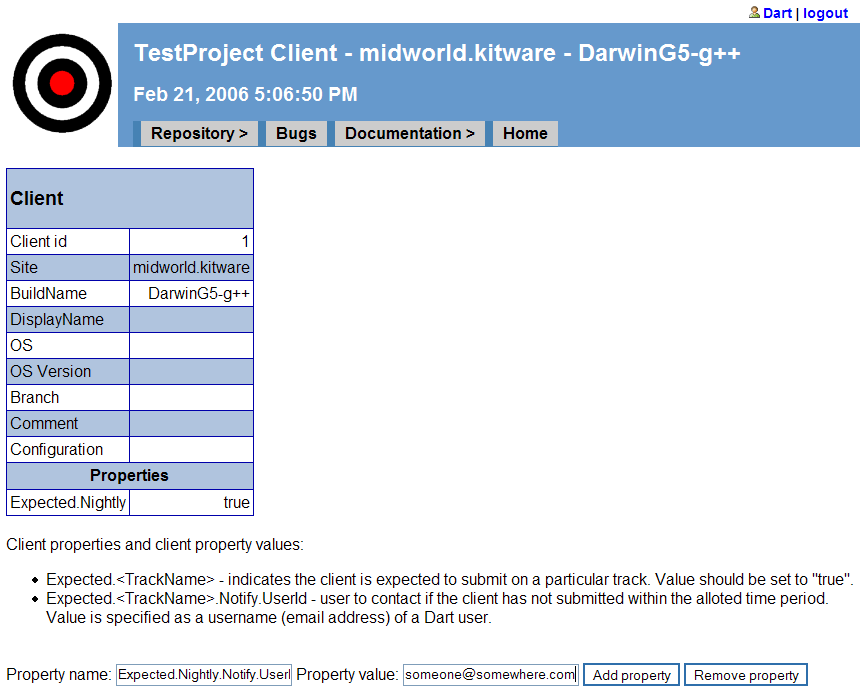
\includegraphics[width=4in]{ClientEnteringNotifyUserId}
	\caption{To assign an owner to a client, assign a client property called \texttt{Expected.<TrackName>.Notify.UserId} a value of a Dart Username (email address).}
	\label{fig:ClientEnteringNotifyUserId}
\end{figure}

\begin{figure}
	\centering
		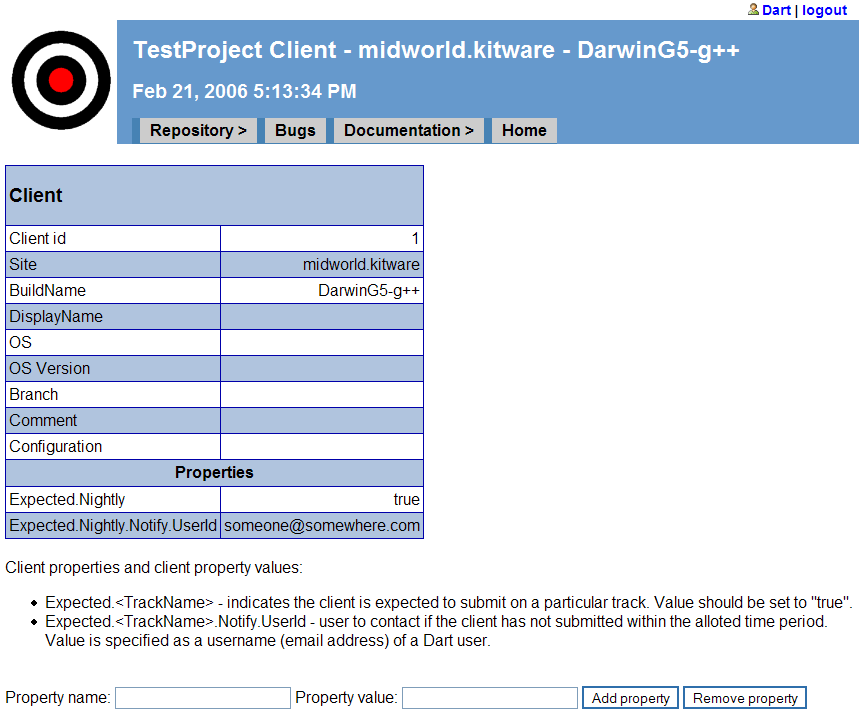
\includegraphics[width=4in]{ClientWithNotifyUserId}
	\caption{Client configured with a Dart User to notify if a submission on the Nightly track is not available.}
	\label{fig:ClientWithNotifyUserId}
\end{figure}


\chapter{Server Setup}
\label{Section:ServerSetup}
\section{Command Line}
The Server has several command line options.
\begin{verbatim}
# java -jar DartServer.jar
usage: DartServer [options] Server.xml <Project0.xml> <Project1.xml> ...
                  <ProjectN.xml>
 -R,--refreshServer       Refresh server resources
 -a,--archive             Archive the project
 -c,--create              Create a new project in the directory specified
 -d,--database            At project creation time, configure the
                          Schema.sql file for generic, Postgres, Derby
 -h,--help                Print help message
 -i,--initialize          Initialize the database from the Schema.sql file
                          in the project directory
 -j,--initializeserver    Initialize the database from the
                          ServerSchema.sql file in the dart server directory
 -k,--createserver        Create a new server in the directory specified
 -l,--logconfiguration    File to configure log4j from, defaults are used
                          if not present
 -r,--refresh             Refresh project resources
 -t,--projecttemplate     Create a new Project using the specified default
                          template: dart/Resources/Server/DartDefault.xml in the jar file is the
                          default
 -u,--upgradeprojectdb    Update all Project's databases to the lastest
                          version
\end{verbatim}

The \texttt{--archive} flag dumps all the Submissions in each project
in Dart XML format into the \texttt{Project/Archive} directory.  This
is the best way to archive a Project all at once.

The \texttt{--projecttemplate} flag is used in conjunction with the
\texttt{--create} argument at project creation time.  If not
specified, the file \filename{dart/Resources/Server/DartDefault.xml} is
used as the Project template.  To extract this file, use the command:
\begin{verbatim}
jar fxv DartServer.jar dart/Resources/Server/DartDefault.xml
\end{verbatim}

The \filename{DartDefault.xml} file may be edited to suit the site
specific needs.  Take care to preserve the FreeMarker tags in the
original file, as they are specific to some parts of the Project creation process.

\section{Server Configuration}
\label{Section:Settings}
In the \texttt{TestServer} directory, there is a file named
\filename{Server.xml}.  This contains the default settings for a dart
server.  The sections of the Server configuration are as follows.

\subsection{Server Info}
\begin{verbatim}
<?xml version="1.0" encoding="utf-8"?>
<Server>
  <Title>TestServer</Title>
  <BaseDirectory>f:\Source\Dart\TestServer</BaseDirectory>
\end{verbatim}

This is the XML preamble followed by the Server information: Title and
BaseDirectory.

\subsection{Ports}
\begin{verbatim}
  <HTTPPort>8081</HTTPPort>
\end{verbatim}
The HTTPPort is used for both serving content and accepting XML-RPC connections.

\subsection{Scheduler}
\begin{verbatim}
  <Scheduler>
    <ThreadPoolSize>10</ThreadPoolSize>
  </Scheduler>
\end{verbatim}

The Scheduler has a default ThreadPoolSize of 10, indicating that 10
 jobs may be executed concurrent by all the Projects managed by this
 Server instance.

\subsection{Database}
\begin{verbatim}
  <!-- Configure the database parameters derby-->
  <Database>
    <!-- Derby database -->
    <Driver>org.apache.derby.jdbc.EmbeddedDriver</Driver>
    <URL>jdbc:derby:f:\Source\Dart\TestServer/Database/TestServer;create=true</URL>
    <ShutdownURL>jdbc:derby:f:\Source\Dart\TestServer/Database/TestServer;shutdown=true
    </ShutdownURL>
    <Username/>
    <Password/>
    <!-- Maximum active / idle connections, -1 is infinite -->
    <MaxActive>10</MaxActive>
    <MaxIdle>3</MaxIdle>
  </Database>
\end{verbatim}

This section specifies the connection to the Server's database.  In
this example, the database is Derby.  The Driver tag specifies the
class implementing the JDBC connection.  URL is the connection string,
ShutdownURL is used to shutdown the Derby database cleanly, it may be
safely left blank for other JDBC packages.  The Username and Password
tags specify the connection parameters.  Dart uses a connection
pooling mechanism for the database with two parameters: MaxActive
specifies the maximum number of active connections, and MaxIdle
specifies the maximum number of idle threads.  If a connection is
needed when MaxActive threads are already active, the connection will
hang until a connection is return to the pool.

\subsection{Servlet Manager}
\begin{verbatim}
  <!-- Servlet configuration -->
  <ServletManager>
    <Servlet>
      <Class>dart.server.servlet.Server</Class>
      <Context>/Dart/*</Context>
      <Properties/>
    </Servlet>
  </ServletManager>
\end{verbatim}

The Servlet manager is responsible for configuring Jetty.  Different
Servlets can respond to different URLs.  In this case, the
dart.server.servlet.Server class is configured to respond to requests
starting with /Dart/*.


\section{Project Configuration}
After following the directions in Section~\ref{Section:QuickStart}, in
the \texttt{TestProject} directory, there is a file named
\filename{Project.xml}.  This is a preconfigured Project configuration
file containing all the settings required to run a basic Dart
Project.  The contents of the file are not presented in their
entirety, but will be discussed section by section.

\subsection{Project Info}
\begin{verbatim}
<?xml version="1.0" encoding="utf-8"?>
<Project>
  <Title>TestProject</Title>
  <BaseDirectory>/projects/Dart/TestProject</BaseDirectory>
\end{verbatim}
The first line is the \texttt{xml} preamble, and is required for all
\texttt{xml} files.  The \xmltag{Project} tag indicates the start of
the Project configuration.  \xmltag{Title} is the project title, and
\xmltag{BaseDirectory} is the absolute path name to the Project
directory.  If the Project is moved to a new location on the file
system, \xmltag{BaseDirectory} must be changed to reflect the new
location.

\subsection{Project Properties}
Certain aspects of a Dart project can be customized by properties
assigned to the project.
\begin{verbatim}
<Properties>
  <Property name="MaxTestsPerSubmission">1500</Property>
  <Property name="RepositoryURL">http://www.itk.org/cgi-bin/viewcvs.cgi/</Property>
  <Property name="RepositoryURL.Type">viewcvs</Property>
  <Property name="RepositoryURL.Repository">Insight</Property>
  <Property name="Menu">
    <![CDATA[
     <ul>
       <li><a href="#">Repository &gt;</a>
         <ul>
          <li><a href="http://www.itk.org/cgi-bin/viewcvs.cgi?cvsroot=Insight">
              Insight</a>
          </li>
          <li>
            <a href="http://www.itk.org/cgi-bin/viewcvs.cgi?cvsroot=InsightApplications">
              Insight Applications
            </a>
          </li>
         </ul>
       <li>
       <li><a href="http://www.itk.org/Bug">Bugs</a></li>
       <li><a href="#">Documentation &gt;</a>
         <ul>
           <li><a href="http://www.itk.org/Insight/Doxygen/html/">Doxygen (API)</a></li>
           <li><a href="http://www.itk.org/">www.itk.org</a></li>
           <li><a href="http://www.itk.org/Wiki/ITK">ITK Wiki</a></li>
           <li><a href="http://www.insightsoftwareconsortium.org/">
               Insight Software Consortium</a>
           </li>
         </ul>
      </li>
      <li><a href="http://www.itk.org/">Home</a></li>
    </ul>
    ]]>
  </Property>
</Properties>
\end{verbatim}

\begin{description}
\item[MaxTestsPerSubmission]{Defines a throttle for the number of tests that can be included in a submission.}
\item[RepositoryURL]{URL for accessing a project's software repository via the web.}
\item[RepositoryURL.Type]{Identifies the type of the web portal for the repository (viewcvs, cvsweb, websvn).}
\item[RepositoryURL.Repository]{Identifies the repository to reference at the specified \texttt{RepositoryURL}}.
\item[Menu]{Definition of a menu to display on web pages.  This menu can include links to navigate within Dart or to navigate to external sites such as documentation, bug trackers, \etc.  \texttt{Menu} is defined as an HTML list (encapsulated in a \texttt{CData} section), with submenus being sublists.  Each menu item is modelled with an \texttt{HREF} within an \texttt{LI}. If a menu item is the title of a submenu, then the \texttt{HREF} should link to ''\#'' and the item label should indicate a drop down menu is available (for instance, suffixing the name with a \texttt{>} sign.  }
\end{description}

\subsection{Database Configuration}
\begin{verbatim}
    <!-- Derby database -->
    <Database>
      <Driver>org.apache.derby.jdbc.EmbeddedDriver</Driver>
      <URL>jdbc:derby:/projects/Dart/TestProject/Database/TestProject;create=true</URL>
      <ShutdownURL>jdbc:derby:/projects/Dart/TestProject/Database/TestProject
                    ;shutdown=true</ShutdownURL>
      <Username/>
      <Password/>
    </Database>
\end{verbatim}
This section configures the Database connection that the Project will
use.  The \xmltag{Driver} tag indicates the JDBC Java class for the
particular type of relational database management system (RDBMS).  In
the example, \texttt{org.apache.derby.jdbc.EmbeddedDriver} is the
driver for the Derby Open Source embedded RDBMS system.  Note: the
\xmltag{ShutdownURL} was broken across two lines for display
purposes, and should not be broken in an actual configuration file.

The \xmltag{URL} tag specifies the connection URL for the RDBMS.
This is a RDBMS specific string.  In the above example, the
\texttt{create=true} property indicates that the driver should create
the database if it does not exist.  Please consult your RDBMS
documentation for the proper setting for the \xmltag{URL} tag.
Because Derby is an embedded RDBMS, it must be properly shutdown to
leave the database in a consistent state.  This is specified in the
\xmltag{ShutdownURL} tag.  If the RDBMS does not require special
shutdown processing, leave this tag empty and it will be ignored.

\xmltag{Username/} and \xmltag{Password} tags specify the
authentication settings for the RDBMS.  In the case of Derby, no
Username/Password is required.

\subsection{CommandManager Configuration}
\begin{verbatim}
  <CommandManager>
    <Command>
      <Name>Submit</Name>
      <Class>dart.server.command.Submit</Class>
      <Properties>
        <Property name="DeleteWhenDigested">true</Property>
      </Properties>
    </Command>
  </CommandManager>
\end{verbatim}
The Dart Server provides an XML-RPC server for results to be
submitted to a Project.  This server operates through a Servlet
configured in the ServletManager (see
Section~\ref{Sec:ServletManager} below).  For the CommandManager to
operate, a dart.server.servlet.CommandServlet object must be added to
the ServletManager.  In addition, the \texttt{CommandServer} can
be configured to respond to any query using specialized
\texttt{Command}s.  The \xmltag{CommandServer} section specifies
the settings for the Project specific settings.

In the instance above, the \xmltag{Command} tag specifies an object
that the Project will use to respond to XML-RPC calls.  Commands must
implement the dart.server.command.Command interface.  \xmltag{Name}
is the object name, \xmltag{Class} is the name of the class that the
CommandManager instantiates and any Properties for the object are
specified using the \xmltag{Properties} tags.  Any public methods of
the object are exposed to XML-RPC calls.

\subsection{ServletManager Configuration}
\label{Sec:ServletManager}
\begin{verbatim}
  <!-- Servlet configuration -->
  <ServletManager>
    <Servlet>
      <Class>dart.server.servlet.Dashboard</Class>
      <Context>/Dashboard/*</Context>
      <Properties>
      </Properties>
    </Servlet>
    <Servlet>
      <Class>dart.server.servlet.Admin</Class>
      <Context>/Admin/*</Context>
      <Properties/>
    </Servlet>
    <Servlet>
      <Class>dart.server.servlet.User</Class>
      <Context>/User/*</Context>
      <Properties/>
    </Servlet>
    <Servlet>
      <Class>dart.server.servlet.ZipServlet</Class>
      <Context>/Zip/*</Context>
      <Properties>
        <!-- Properties for the ZipServlet are encodings for the files
             in the zip archive.  The name of the property is used to match the
             suffix of the file (lowercased...).
             .html == text/html, .png == image/png
             -->
        <Property name=".html">text/html</Property>
        <Property name=".htm">text/html</Property>
        <Property name=".xml">text/xml</Property>
        <Property name=".xsl">text/xml</Property>
        <Property name=".png">image/png</Property>
        <Property name=".jpg">image/jpg</Property>
        <Property name=".jpeg">image/jpg</Property>
        <Property name=".css">text/css</Property>
        <Property name=".js">application/x-javascript</Property>
        <Property name=".txt">text/plain</Property>
      </Properties>
    </Servlet>
    <Servlet>
      <Class>dart.server.servlet.CommandServlet</Class>
      <Context>/Command/</Context>
      <Properties/>
    </Servlet>
    <Servlet>
      <Class>dart.server.servlet.ChartServlet</Class>
      <Context>/Chart</Context>
      <Properties/>
    </Servlet>
  </ServletManager>
\end{verbatim}
To generate Dashboard pages, the Server uses the Jetty Servlet
engine in conjunction with the FreeMarker template engine.  Stock
Project Servlets are automatically configured at project creation
time.  User defined Servlets may be added if desired.  The
\xmltag{Class} tag indicates the class of the Servlet,
\xmltag{Context} tag indicates how the Servlet is found by Jetty.
By default, the Project title is stored in the Servlet's initial
parameters as \texttt{"project"} and may be accessed as
\texttt{getInitParameter ( "project" ) } within the Servlet.
Parameters in the \xmltag{Properties} section are also put in the
initial parameters map.

The second servlet in the stock configuration web access to administer
a project. Users in the roles of \texttt{Dart.Administrator}
and \emph{ProjectName}.\texttt{Administrator} will have access to the 
administration tools from their \emph{User} page.  

The third servlet in the stock configuration provides \emph{User}
logins and \emph{User} configuration.

The forth servlet in the stock configuration provides cabilities to serve
content from within zip archives.  Some third party software analysis tools 
output web-based reports.  These web-based reports can be place in a zip
archive and placed on the Dart server.  The Dart server can serve pages 
from the web-based report as if the pages were unarchived on the Dart server.

The fifth Servlet in the stock configuration is
dart.server.servlet.CommandServlet.  CommandServlet accepts XML-RPC
calls and delegates them to the appropriate handler object as
configured in the CommandManager.  The last Servlet is the
ChartServlet used to generate charts for the dashboard.

To call an XML-RPC method, the URL needed is determined by the root
project URL, \ie
\texttt{http://localhost:8081/\emph{ProjectName}/Command/\emph{Command}.\emph{Method}}.
 For example, the URL to submit some results to the Dart project
TestProject running on the local system is:
\url{http://localhost:8081/TestProject/Command/} and the method is \texttt{Submit.put}.

The sixth servlet in the stock configuration provides Dart with charting and plotting 
capabilities.  The \emph{ChartServlet} uses JFreeChart to generate plots of test timings and status.



\subsubsection{Adding a new servlet to Dart}
\label{Sec:UserServlet}

If you are building Dart from source, you can add additional servlets 
to the DartServer.jar by adding the servlet's source code to 
\filename{Dart/Source/dart/server/servlet} directory and rebuilding.  The
servlet can be activated for a project as in the above example.

If you are running from a pre-built DartServer.jar, you can still add
additional servlets to Dart. This is done by adding the \texttt{classpath} 
property to the servlet definition in the Project.xml file.
\begin{verbatim}
    <Servlet>
      <Class>user.servlet.MyDashboard</Class>
      <Context>/MyDashboard/*</Context>
      <Properties>
        <Property name="Foo">10</Property>
        <Property name="classpath">foo.jar</Property>
      </Properties>
    </Servlet>
\end{verbatim}

This example adds the class \texttt{user.servlet.MyDashboard} from the \filename{foo.jar} 
archive to the project and assigns it the url space of \texttt{/MyDashboard/*}.

\subsection{MessengerManager Configuration}
\label{Section:MessengerManager}
\begin{verbatim}
  <MessengerManager>
    <Messenger>
      <Name>SMTP</Name>
      <Type>dart.server.messenger.SMTPMessenger</Type>
      <!-- The properties specified on the SMTPMessenger are passed directly 
           to JavaMail to configure the mail host, port, protocols, 
           authentication, encryption, etc. -->
      <Properties>
        <Property name="mail.host">localhost</Property>
        <Property name="mail.port">25</Property>
        <Property name="mail.from">dart@localhost</Property>
        <Property name="mail.transport.protocol">smtp</Property>
      </Properties>
    </Messenger>
  </MessengerManager>
\end{verbatim}

The MessengerManager allows for different messaging systems to be employed by Dart. Currently, only an SMTPMessenger is provided. In the future, a variety of messaging services may be available, for instance, instance messaging and pager messaging.

The SMTPMessenger uses the same property names as JavaMail and these properties are passed directly to a JavaMail provider. Authenticated and secure connections to the 
SMTP provider will be available in future versions of Dart.

Multiple Messengers of the same type can be configured.  For instance, a Project may use different SMTPMessenger's to report on different Events.  One SMTPMessenger may be configured to be used when a submission contains information on build errors while another SMTPMessenger with a different \emph{from} address could be used to report on server level issues.

\subsection{ListenerManager Configuration}
\label{Section:ListenerManager}
\begin{verbatim}
  <!-- Listener manager.  Do specific things when events happen in the Project -->
  <ListenerManager>
    <Listener>
      <Type>dart.server.listener.SubmissionErrorsListener</Type>
      <Properties>
        <Property name="Messenger">SMTP</Property>
      </Properties>
    </Listener>
    <Listener>
      <Type>dart.server.listener.MissingSubmissionListener</Type>
      <Properties>
        <Property name="Messenger">SMTP</Property>
      </Properties>
    </Listener>
  </ListenerManager>
\end{verbatim}

While a Dart Project is running, different Events of note may
occur.  The ListenerManager receives Events from the Project and
triggers each Listener that can handle the event. 
queries each Listener to see if the Listener can handle the event.
Some Listeners may specify a Messenger  for transmitting information 
about the event to registered Users.

The first Listener in the stock configuration determines whether a
submission contains information about build errors and notifies the 
authors of the code tested in the submission.  The authors of the code in the submission are determined from the \texttt{Update} information sent to the Dart server. Each
author that can be linked to a Dart User is notified via email with a link
to a web page summarizing the submission. More information on Dart Users can be found in Section~\ref{Section:Users}.

The second Listener in the stock configuration determines whether any
clients that are expected to submit on a particular track have yet to submit to the dashboard within the allotted timeframe.  More details on configuring \emph{when} a submission is noted as being missing is in Section~\ref{Section:TaskConfiguration}.
More information of configuring a client as being \emph{expected} can be found in Section~\ref{Section:ClientConfiguration}.
 

\subsection{Task Configuration}
\label{Section:TaskConfiguration}
\begin{verbatim}
  <!-- Scheduled tasks.  The Schedule tag is in cron format. -->
  <Task>
    <Type>dart.server.task.QueueManager</Type>
    <Schedule>0 0/10 * * * ?</Schedule>
    <Properties>
      <Property name="MaxTasks">10</Property>
    </Properties>
  </Task>
\end{verbatim}

Tasks configured in the \filename{Project.xml} file are periodically
scheduled.  Tasks must implement the \texttt{dart.server.task.Task}
interface.  In the above example, the
\texttt{dart.server.task.QueueManager} is scheduled to run every 10
minutes.  The \texttt{QueueManager} class processes other Tasks that have been
placed in the TaskQueue.  The \texttt{Properties} tag specifies
settings that are passed into the Task when it executes.  For
\texttt{QueueManager}, the ``MaxTasks'' property indicates how many
queued tasks will be processed at during each execution, providing a
``throttling'' mechanism.  

One task that is scheduled after each submission is received by the server is the 
XMLResultProcessor task.  This task performs the XML parsing of a submission
and populates the Project database so the information can be displayed on the
Dashboard. Since the XML processing is scheduled as a task after a submission 
is received, there is an inherent delay between the submission being received
and when the data in the submission is available for display on the Dashboard.
To reduce this delay, you can change the schedule of the QueueManager task.
By default, the QueueManager runs every 10 minutes.  You may want to reduce the schedule
of the QueueManager task to run every few seconds.


\begin{verbatim}
    <Task>
      <!-- Reindex Tracks if the definition has changed every night at 2am -->
      <Type>dart.server.task.ReindexTrackTask</Type>
      <Schedule>0 0 2 * * ?</Schedule>
      <Properties/>
    </Task>
\end{verbatim}

The ReindexTrackTask visits all existing Tracks in the database.  A
Track is deleted and the Submissions contained in it are reindexed if
(1) the Track definition has been removed from \filename{Project.xml},
(2) if the Track does not contain any Submissions, (3) if the Track
has changed duration.  This is scheduled to occur at 2am each day.

\begin{verbatim}
    <Task>
      <Type>dart.server.task.MissingSubmissionTask</Type>
      <!-- Check for missing submissions from 5am to 9pm (exclusive) 
           every 15 minutes.  Since the Nightly track starts at 9pm, 
           this gives 8 hours for submissions to roll in before they are 
           marked as late -->
      <Schedule>0 */15 5-20 * * ?</Schedule>
      <Properties>
        <!-- What track to monitor -->
        <Property name="Track">Nightly</Property>
      </Properties>
    </Task>
\end{verbatim}

The MissingSubmissionTask checks whether clients that have been marked
as \emph{expected} have submitted to the Dashboard.  If any \emph{expected}
clients have not submitted, a \texttt{MissingSubmissionEvent} is triggered.
The MissingSubmissionListener will process this event and notify the 
Dart Users associated with a particular client.  The task above is configured to start running 8 hours after the \texttt{Nightly} track starts and checks every 15 minutes for missing submissions. More information on configuring
\emph{expected} submissions can be found in Section~\ref{Section:ClientConfiguration}.

The format of the \xmltag{Schedule} tag
is detailed at
\texttt{http://quartz.sourceforge.net/javadoc/org/quartz/CronTrigger.html}
and is reproduced here for clarity.

\subsubsection{Cron Expressions}
 For those unfamiliar with ``cron'', this means being able to create a firing schedule such as: ``At 8:00am every Monday through Friday'' or ``At 1:30am every last Friday of the month''.

A ``Cron-Expression'' is a string comprised of 6 or 7 fields separated
by white space. The 6 mandatory and 1 optional fields are as follows:

\begin{tabular}{lll}
Field Name &            Allowed Values &                Allowed Special Characters \\
\hline
Seconds &               0-59 &          , - * /   \\ 
Minutes&                0-59&           , - * / \\
Hours&          0-23&           , - * / \\
Day-of-month&           1-31&           , - * ? / L W C \\
Month&          1-12 or JAN-DEC&                , - * / \\
Day-of-Week&            1-7 or SUN-SAT&                 , - * ? / L C \# \\
Year (Optional)&                empty, 1970-2099&               , - * / \\
\end{tabular}

The ``*'' character is used to specify all values. For example, ``*'' in
the minute field means ``every minute''.

The ``?'' character is allowed for the day-of-month and day-of-week
fields. It is used to specify 'no specific value'. This is useful when
you need to specify something in one of the two fields, but not the
other. See the examples below for clarification.

The ``-'' character is used to specify ranges For example ``10-12'' in the
hour field means ``the hours 10, 11 and 12''.

The ``,'' character is used to specify additional values. For example
``MON,WED,FRI'' in the day-of-week field means "the days Monday,
Wednesday, and Friday".

The ``/'' character is used to specify increments. For example ``0/15'' in
the seconds field means ``the seconds 0, 15, 30, and 45''. And ``5/15'' in
the seconds field means ``the seconds 5, 20, 35, and 50''. You can also
specify ``/'' after the ``*'' character - in this case ``*'' is equivalent
to having ``0'' before the ``/''.

The ``L'' character is allowed for the day-of-month and day-of-week
fields. This character is short-hand for ``last'', but it has different
meaning in each of the two fields. For example, the value ``L'' in the
day-of-month field means ``the last day of the month'' - day 31 for
January, day 28 for February on non-leap years. If used in the
day-of-week field by itself, it simply means ``7'' or ``SAT''. But if used
in the day-of-week field after another value, it means ``the last xxx
day of the month'' - for example ``6L'' means "the last friday of the
month". When using the ``L'' option, it is important not to specify
lists, or ranges of values, as you'll get confusing results.

The ``W'' character is allowed for the day-of-month field. This
character is used to specify the weekday (Monday-Friday) nearest the
given day. As an example, if you were to specify ``15W'' as the value
for the day-of-month field, the meaning is: "the nearest weekday to
the 15th of the month". So if the 15th is a Saturday, the trigger will
fire on Friday the 14th. If the 15th is a Sunday, the trigger will
fire on Monday the 16th. If the 15th is a Tuesday, then it will fire
on Tuesday the 15th. However if you specify ``1W'' as the value for
day-of-month, and the 1st is a Saturday, the trigger will fire on
Monday the 3rd, as it will not 'jump' over the boundary of a month's
days. The ``W'' character can only be specified when the day-of-month is
a single day, not a range or list of days.

The ``L'' and ``W'' characters can also be combined for the day-of-month
expression to yield ``LW'', which translates to "last weekday of the
month".

The ``\#'' character is allowed for the day-of-week field. This character
is used to specify ``the nth'' XXX day of the month. For example, the
value of ``6\#3'' in the day-of-week field means the third Friday of the
month (day 6 = Friday and ``\#3'' = the 3rd one in the month). Other
examples: ``2\#1'' = the first Monday of the month and ``4\#5'' = the fifth
Wednesday of the month. Note that if you specify ``\#5'' and there is not
5 of the given day-of-week in the month, then no firing will occur
that month.

The ``C'' character is allowed for the day-of-month and day-of-week
fields. This character is short-hand for ``calendar''. This means values
are calculated against the associated calendar, if any. If no calendar
is associated, then it is equivalent to having an all-inclusive
calendar. A value of ``5C'' in the day-of-month field means ``the first
day included by the calendar on or after the 5th''. A value of ``1C'' in
the day-of-week field means "the first day included by the calendar on
or after sunday".

The legal characters and the names of months and days of the week are
not case sensitive.

Here are some full examples:

\begin{tabular}{lp{12cm}}
Expression&             Meaning\\
\hline
``0 0 12 * * ?''          &Fire at 12pm (noon) every day \\
``0 15 10 ? * *''                 &Fire at 10:15am every day \\
``0 15 10 * * ?''                 &Fire at 10:15am every day \\
``0 15 10 * * ? *''               &Fire at 10:15am every day \\
``0 15 10 * * ? 2005''            &Fire at 10:15am every day during the
year 2005 \\
``0 * 14 * * ?''          &Fire every minute starting at 2pm and ending
at 2:59pm, every day \\
``0 0/5 14 * * ?''                &Fire every 5 minutes starting at 2pm
and ending at 2:55pm, every day \\
``0 0/5 14,18 * * ?''             &Fire every 5 minutes starting at 2pm
and ending at 2:55pm, AND fire every 5 minutes starting at 6pm and
ending at 6:55pm, every day \\
``0 0-5 14 * * ?''                &Fire every minute starting at 2pm and
ending at 2:05pm, every day \\
``0 10,44 14 ? 3 WED''            &Fire at 2:10pm and at 2:44pm every
Wednesday in the month of March. \\
``0 15 10 ? * MON-FRI''           &Fire at 10:15am every Monday,
Tuesday, Wednesday, Thursday and Friday \\
``0 15 10 15 * ?''                &Fire at 10:15am on the 15th day of
every month \\
``0 15 10 L * ?''                 &Fire at 10:15am on the last day of
every month \\
``0 15 10 ? * 6L''                &Fire at 10:15am on the last Friday of
every month \\
``0 15 10 ? * 6L''                &Fire at 10:15am on the last Friday of
every month \\
``0 15 10 ? * 6L 2002-2005''              &Fire at 10:15am on every last
friday of every month during the years 2002, 2003, 2004 and 2005 \\
``0 15 10 ? * 6\#3''              &Fire at 10:15am on the third Friday
of every month \\
\end{tabular}

Pay attention to the effects of ``?'' and ``*'' in the day-of-week and day-of-month fields!

NOTES:
\begin{itemize}
    \item Support for the features described for the ``C'' character is not complete.
    \item Support for specifying both a day-of-week and a day-of-month value is not complete (you'll need to use the ``?'' character in on of these fields).
    \item Be careful when setting fire times between mid-night and
1:00 AM - ``daylight savings'' can cause a skip or a repeat depending on
whether the time moves back or jumps forward.
\end{itemize}

Another example Task is the \texttt{SaveStatistics} Task which writes
the Project statistics to the file system on a regular bases.  The Task
does not have any parameters, and saves the statistics in a file named
\texttt{Statistics.txt} in the Project directory.
\begin{verbatim}
  <Task>
    <Type>dart.server.task.SaveStatistics</Type>
    <Schedule>0 * * * * ?</Schedule>
    <Properties>
    </Properties>
  </Task>
\end{verbatim}


An extremely important Task is the ArchiveTask.  This Task is detailed
in Section~\ref{Section:ArchiveTask}.

\subsection{Task List}
These are the currently available Tasks:
\begin{description}
  \item[ArchiveTask] The ArchiveTask is responsible for finding old
  data in removing it from the Project, potentially archiving the data
  to the filesystem.
  \item[DeleteDataTask] The DeleteDataTask is used internally by the
  ArchiveTask.  It is responsible for deleting files from the Project,
  if they are no longer referenced in the database.
  \item[GarbageCollectionTask] The GarbageCollectionTask simply runs
  the Java garbage collector.
  \item[MissingSubmissionTask] The MissingSubmissionTask determines whether any clients have been marked as expected and checks whether these clients have submitted to the Dashboard within the allotted time period.  Users registered as maintainers of the clients which have not submitted will be notified via email.
  \item[PlaceSubmissionInTrackTask] The PlaceSubmissionInTrackTask
  determines which Track a Submission belongs to and places it there.
  This Task should only be used internally and is queued by the
  XMLResultProcessor as configured in Section~\ref{Section:RollupManager}.
  \item[QueueManager] This is the most important Task.  The
  QueueManagerTask pulls queued Tasks from the TaskQueue table and
  executes them.  The QueueManager is scheduled to run every 10
  minutes by default~(see Section~\ref{Section:TaskConfiguration}).
  \item[SaveStatistics] The SaveStatistics Task writes out the
  Project's statistics to disk~(see Section~\ref{Section:TaskConfiguration}).
  \item[SummarizeBuildTask] The SummarizeBuildTask
  collects and rolls up summary information for a build.
  This Task should only be used internally and is queued by the
  XMLResultProcessor as configured in Section~\ref{Section:RollupManager}.
  \item[SummarizeCoverage] The SummarizeCoverageTask
  collects and rolls up coverage summary information.
  This Task should only be used internally and is queued by the
  XMLResultProcessor as configured in Section~\ref{Section:RollupManager}.
  \item[SummarizeDynamicAnalysis] The SummarizeDynamicAnalysis
  collects and rolls up Dynamic Analysis summary information for a Submission
  This Task should only be used internally and is queued by the
  XMLResultProcessor as configured in Section~\ref{Section:RollupManager}.
  \item[SummarizeTests] The SummarizeTests
  collects and rolls up Test summary information for a build.
  This Task should only be used internally and is queued by the
  XMLResultProcessor as configured in Section~\ref{Section:RollupManager}.
  \item[Task] Task is the interface that each Task in this list implements.
  \item[XMLResultProcessor] The XMLResultProcessor is queued when a
  Submission is pushed to the server.  This Task parses the XML file
  and puts the Submission data into the database.  The
  XMLResultProcessor uses the RollupManager configuration as set in
  Section~\ref{Section:RollupManager} to queue further Tasks.
\end{description}

\subsection{TrackManager}
\label{Section:TrackManager}
Submissions are grouped and navigated by a collection of \emph{Tracks}. You define  
tracks for a project by configuring the TrackManager. TemporalTracks group submissions
that pertain to a common interval of time.  Multiple Tracks can be configured to serve
different types of submissions and review processes.

\begin{verbatim}
  <TrackManager>
    <DefaultTrack>Nightly</DefaultTrack>
    <TemporalTrack>
      <Name>Nightly</Name>
      <Start>9:00 PM</Start>
      <Duration>24</Duration>
      <Priority>0</Priority>
      <DefaultSortBy>buildName</DefaultSortBy>
      <DefaultOrder>ascending</DefaultOrder>
    </TemporalTrack>

    <TemporalTrack>
      <Name>Continuous</Name>
      <Start>9:00 PM</Start>
      <!-- Duration is in floating point hours -->
      <Duration>24</Duration>
      <DefaultSortBy>timeStamp</DefaultSortBy>
      <DefaultOrder>descending</DefaultOrder>
    </TemporalTrack>

    <TemporalTrack>
      <Name>Experimental</Name>
      <Start>9:00 PM</Start>
      <!-- Duration is in floating point hours -->
      <Duration>24</Duration>
      <DefaultSortBy>timeStamp</DefaultSortBy>
      <DefaultOrder>descending</DefaultOrder>
    </TemporalTrack>

    <TemporalTrack>
      <Name>Weekly</Name>
      <Start>Jan 16, 2005 9:00 PM</Start>
      <!-- Duration is in floating point hours -->
      <Duration>168</Duration>
      <DefaultSortBy>buildName</DefaultSortBy>
      <DefaultOrder>ascending</DefaultOrder>
    </TemporalTrack>
  </TrackManager>
\end{verbatim}

In the above configuration, four tracks are defined: Nightly, Continuous, Experimental, and Weekly.
The Nightly track is labeled by the configuration as the default track.  The default track will collect any submission that is not designated for a specific  track. The Nightly, Continuous, and
Experimental tracks are configured to start a 9:00PM in the timezone of the server and collect submissions
that fall within a 24 hour period. The Weekly track is configured to collect submissions over a 
span of a week.  Note, that tracks do not have to span the duration of time.  For instance, you may want to
configure the Continuous track to only span a 4 hour window, thereby limiting the number of submissions displayed on dashboard. 

Tracks will appear on the Dashboard in the order they are specified in Project.xml.  The ordering 
can be changed by specifying a \xmltag{Priority}. 

TemporalTrack's have two other optional parameters \xmltag{DefaultSortBy} and \xmltag{DefaultOrder}.  These parameters control how the display of submissions for the track appear on the dashboard. \xmltag{DefaultSortBy} specifies how submissions are sorted on the dashboard.  \xmltag{DefaultSortBy} can have values of:
\begin{itemize}
\item site
\item buildName
\item updateCount
\item errorCount
\item warningCount
\item elapsedBuildTime
\item passedCount
\item failedCount
\item notRunCount
\item elapsedTestTime
\item timeStamp
\end{itemize}
\xmltag{DefaultOrder} can have values of ``ascending'' or ``descending''.

CTest (see Section~\ref{Section:CTest}) uses a standard collection of Tracks: Nightly, Continuous, and Experimental. If you are using CTest for a Dart client, you should define your tracks to be Nightly, Continuous, and Experimental.


\subsection{RollupManager}
\label{Section:RollupManager}
After a Submission is process and the raw data placed in the database,
the configuration in the RollupManager section of the Project.xml file
controls which Tasks the XMLResultProcessor queues to summarize and
further process the Submission's data.  When queued, the Task is given
a the SubmissionId through the \texttt{SubmissionId} Property.  The
default RollupManager configuration is below, each Task may be given a
set of Properties, and is queued with the \texttt{Priority} given by
the tag.

\begin{verbatim}
  <RollupManager>
    <Rollup>
      <Type>dart.server.task.SummarizeTests</Type>
      <Priority>4</Priority>
      <Properties/>
    </Rollup>
    <Rollup>
      <Type>dart.server.task.SummarizeBuildTask</Type>
      <Priority>4</Priority>
      <Properties/>
    </Rollup>
    <Rollup>
      <Type>dart.server.task.SummarizeCoverage</Type>
      <Priority>4</Priority>
      <Properties/>
    </Rollup>
    <Rollup>
      <Type>dart.server.task.SummarizeDynamicAnalysis</Type>
      <Priority>4</Priority>
      <Properties/>
    </Rollup>
    <Rollup>
      <Type>dart.server.task.PlaceSubmissionInTrackTask</Type>
      <Priority>4</Priority>
      <Properties/>
    </Rollup>
    <Rollup>
      <!-- Note, the SubmissionEvent must be the last Task -->
      <Type>dart.server.event.SubmissionEventTask</Type>
      <Priority>5</Priority>
      <Properties/>
    </Rollup>
  </RollupManager>
\end{verbatim}

\section{Events}
\label{Section:Events}

While the Dart server is running, various interesting events may
occur; \eg Nightly Submissions present/absent, low disk space, build
failures, \etc.  To monitor and respond to Events, the Dart Server may
be configured with different Listeners that receive Events and have
the opportunity to respond in a variety of ways.  The Event subsystem
has two components, Event sources and Listeners.  Events are generated
automatically (and programatically) by the Dart Server and are handled
immediately by the ListenerManager.  The ListenerManager checks each
Listener defined by the Project, if a Listener is registered for the particular type of Event, the Listener's trigger method
is called.  The Listener is free to take any action based on the
contents of the Event, but is not allowed to modify the Event in any
way.

Currently defined Events:
\begin{description}
\item[SubmissionEvent] This Event is triggered by the RollupManager
after all the other Rollups have been done.  This Event signifies that
a Submission has been completely processed.
\item[MissingSubmissionEvent] This Event is triggered by the MissingSubmissionTask. This events signifies that certain clients were expected to submit to the Dashboard on a particular track but these clients have yet to perform a submission.  This event may indicate a problem withe client or the network between the client and the Dart server.
\end{description}


Currently defined Listeners:
\begin{description}
\item[SubmissionErrorsListener]  This Listener determines if a
Submission is of a particular type and sends the appropriate email to
the list of registered Users.
\item[MissingSubmissionListener] This Listener notifies Users registered with a client that said client has yet to submit to the Dashboard.
\end{description}

\section{Archiving a Dart Server}
\label{Section:ArchiveTask}

Though the ArchiveTask strictly belongs in the Task section of the
configuration file, it's options are quite complex and deserve a
section of it's own.  The basic job of the ArchiveTask is to copy data
from the Dart database to the file system in a easy to restore format
and, optionally, delete the data from the database.



A project can have 0 or more ``Archivers''.  Each Archiver selects a set
of Submissions that matches some criteria.  The current selection criteria are:

\begin{itemize}
\item AgeInDays  A submission must be older than this to be considered (may be BuildStamp or CreatedTimeStamp[when the submission happened])
\item MatchTrack a comma seperated list of regular expressions to match against the track of each Submission
\item MatchSite a comma seperated list of regular expressions to match against the Site
\item MatchBuildName a comma seperated list of regular expressions to match against the BuildName
\item MatchTest a comma seperated list of regular expressions to match
against each test in the submission
\end{itemize}


Once a submission is matched, it is archived, if not already archive, to a user specified directory (default is ProjectDirectory/Archive).  When the ``Working'' directory reaches a specific size (MaxDirectorySizeMB default is 700), it is renamed using the current date time stamp and a new Working directory is created.  In this way, a set of 700MB directories is created and may be safely moved to CDROM or other archival media and deleted.

Each Archiver has specified levels of archive, specified by the ArchiveLevel:

\begin{itemize}
\item 0 default, all data is still in the Database
\item 1 remove least amount of data.  All bulk data (images, logs, \etc) are to be removed
\item 2 remove all leaf tests and data, leaving only intermediate levels in the Test hierarchy
\item 3 remove all non-root Tests, leaving rollup info at the root level of the Test hierarchy
\item 4 remove all data and the Submission itself.  This is as if the submission had never existed
\end{itemize}

This is an example of an ArchiveTask definition:
\begin{verbatim}
  <Task>
    <!-- Archive task, runs at 3am each morning -->
    <Type>dart.server.task.ArchiveTask</Type>
    <Schedule>*/30 * * * * ?</Schedule>
    <Properties>
      <Property name="ArchiverList">Nightly</Property>

      <Property name="Archiver.Nightly.WriteArchive">true</Property>
      <Property name="Archiver.Nightly.FileNamePattern">Archive-%L-%P-%S-%B-%T-%D.xml.gz</Property>
      <Property name="Archiver.Nightly.Template">ArchiveSubmission.xml</Property>
      <Property name="Archiver.Nightly.MatchTrack">.*</Property>
      <Property name="Archiver.Nightly.AgeInDays">0.010</Property>
      <Property name="Archiver.Nightly.ArchiveLevel">3</Property>
      <Property name="Archiver.Nightly.MatchTest">.*</Property>
      <Property name="Archiver.Nightly.MatchSite">.*</Property>
      <Property name="Archiver.Nightly.ArchiveBy">CreatedTimeStamp</Property>
      <Property name="Archiver.Nightly.MaxDirectorySizeMB">700</Property>
      <Property name="Archiver.Nightly.ArchiveDirectory">/tmp/DartArchive</Property>
      
    </Properties>
  </Task>
\end{verbatim}
This tag defines the list of Archivers (comma separated).  So we only
have one called ``Nightly''
\begin{verbatim}
      <Property name="ArchiverList">Nightly</Property>
\end{verbatim}
Each Archiver is run in the order of the ArchiverList Property.


All properties for this Archiver are indicated by ``Archiver.Foo.PropertyName'' where Foo is the name of the property.  For example: ``Archiver.Nightly.AgeInDays''.  Below, when I refer to a Property, it is assumed there is a ``Archiver.Nightly.'' prefix to it.  So ArchiveLevel really refers to ``Archiver.Nightly.ArchiveLevel''.

The first check is to see match Submissions by AgeInDays.  In this
case, 0.010 is about 10 minutes.  The Database column to match is the
CreatedTimeStamp.  This is when the submission hit the Dart Server.
The other option for ArchiveBy is TimeStamp, which is the datetime
reported by the Client.  The last criteria is that the Submission must
have an ArchiveLevel less than the one specified for this Archiver
(this is explained below).  Thus to match, a Submission must be older
than 0.01 days by CreatedTimeStamp, and have an archive level of < 3.
\begin{verbatim}
      <Property name="Archiver.Nightly.AgeInDays">0.010</Property>
      <Property name="Archiver.Nightly.ArchiveBy">CreatedTimeStamp</Property>
      <Property name="Archiver.Nightly.ArchiveLevel">3</Property>
\end{verbatim}

From the list of Submissions return, each is examined in turn.  The
first test is by Site and BuildStamp:
\begin{verbatim}
      <Property name="Archiver.Nightly.MatchSite">.*</Property>
      <Property name="Archiver.Nightly.MatchBuildName">.*</Property>
\end{verbatim}

MatchSite is a comma separated list of regular expressions.  ``.*''
matches all sites.  If the Submission does not match any of the
expressions, it is ignored.  The same matching is applied for
MatchBuildName.

The next test is to Match the Track:
\begin{verbatim}
      <Property name="Archiver.Nightly.MatchTrack">.*</Property>
\end{verbatim}

Again, a comma separated list.  Here we match all tracks.

If a Submission matches by Site, Track and BuildName, the Submission's ArchiveDateStamp and ArchiveLevel are examined.  If ArchiveDateStamp is null, then go ahead and archive the Submission to disk as outlined below.  If the CreatedTimeStamp is later than the ARchiveDateStamp, some new data has hit the database since the last archive, so go ahead and archive the Submission to disk.

To archive to Disk, the Archiver writes all the Submission data to one
big XML file using the new Dart v2 XML format.  This is specified as a
FreeMarker template by this Property.
\begin{verbatim}
      <Property name="Archiver.Nightly.Template">ArchiveSubmission.xml</Property>
\end{verbatim}

ArchiveSubmission.xml is the default.  This file is suitable for re-submitting to the Dart Server.  However, if the WriteArchive property is false, the data will not be written to disk.  This is useful for Experimental and continuous builds that you may not care about.  ``true'' is the default.
\begin{verbatim}
      <Property name="Archiver.Nightly.WriteArchive">true</Property>
\end{verbatim}

Once the file has been generated, it is written to disk.  Each Archiver has a location to write to.  The default is the ``ProjectDirectory/Archive'' directory that is created when the project starts up.  In our case we write to /tmp/DartArchive:
\begin{verbatim}
      <Property name="Archiver.Nightly.ArchiveDirectory">/tmp/DartArchive</Property>
\end{verbatim}

Inside /tmp/DartArchive two directories will be created: Working and Temporary.  Once the XML is generated in Temporary, it is gzipped and moved to Working.  The filename is generated by this Property:
\begin{verbatim}
<Property name="Archiver.Nightly.FileNamePattern">Archive-%L-%P-%S-%B-%T-%D.xml.gz</Property>

Where: 
           %L is replaced by ArchiveLevel
           %P is replaced by the project name
           %S is replaced by the Site name
           %B is replaced by the BuildName
           %T is replaced by the TrackName
           %D is replaced by the DateTimeStamp
           %N is replaced by the current time "now" in UTC
\end{verbatim}

So you can have as much or as little info encoded in the filename as you like.

If moving the file from Temporary would push the Working Directory over the limit set by:
\begin{verbatim}
      <Property name="Archiver.Nightly.MaxDirectorySizeMB">700</Property>
\end{verbatim}

The Working directory is renamed by the current time in UTC and a new Working directory is started.  We could specify that the Working directory is rolled over on a regular time schedule rather than a file size criteria if that would be useful.

Finally, the Archiver decides which data from the Submission to remove (since it's all been archived by now).  This is decided by ArchiveLevel
\begin{verbatim}
      <Property name="Archiver.Nightly.ArchiveLevel">3</Property>
\end{verbatim}

 ArchiveLevel indicates how much data to remove
\begin{itemize}
             \item 1 remove least amount of data.  All bulk data (images, logs, \etc) are to be removed
             \item 2 remove all leaf tests and data, leaving only intermediate levels in the Test hierarchy
             \item 3 remove all non-root Tests, leaving rollup info at the root level of the Test hierarchy
             \item 4 remove all data and the Submission itself
\end{itemize}

Each Test is matched using the MatchTest Property:
\begin{verbatim}
      <Property name="Archiver.Nightly.MatchTest">.*</Property>
\end{verbatim}

Except at level 4, where everything is removed.  If a test does not match, it is ignored and no data is deleted from it.

Finally, the Submission's ArchiveLevel is updated, as is the ArchivedTimeStamp.  Now this Submission will not match the initial select, as it's ArchiveLevel is equal to the ArchiveLevel for this Archiver.

The Archiver then processes the next Submission until no more are found.

\subsection{Default Archivers}
By default, several Archivers are defined in the Project, however the
Archivers are not active.  They are:
\begin{itemize}
           \item Nightly {
\begin{itemize}
\item Level 1 after 2 months (NightlyLevel1)
\item Level 2 after 4 months (NightlyLevel2)
\item Level 3 after 6 months (NightlyLevel3)
\end{itemize}
}
           \item Continuous {
\begin{itemize}
\item Level 2 after 1 week (ContinuousLevel2)
\item Level 4 after 1 month (ContinuousLevel4)
\end{itemize}
}
           \item Experimental {
\begin{itemize}
\item Level 4 after 1 week - No files saved (ExperimentalLevel4)
\end{itemize}
}
\end{itemize}

To enable the default Archivers, uncomment this line(broken for clarity):
\begin{verbatim}
<!--
  <Property name="ArchiverList">NightlyLevel1,NightlyLevel2,NightlyLevel3,
        ContinuousLevel2,ContinuousLevel4,ExperimentalLevel4</Property>
-->
\end{verbatim}

The definition of the default Archivers are:
\begin{verbatim}
      <!-- Nightly archivers -->
      <Property name="Archiver.NightlyLevel1.AgeInDays">60</Property>
      <Property name="Archiver.NightlyLevel1.ArchiveLevel">1</Property>
      <Property name="Archiver.NightlyLevel1.MatchTrack">Nightly</Property>

      <Property name="Archiver.NightlyLevel2.AgeInDays">120</Property>
      <Property name="Archiver.NightlyLevel2.ArchiveLevel">2</Property>
      <Property name="Archiver.NightlyLevel2.MatchTrack">Nightly</Property>
      
      <Property name="Archiver.NightlyLevel3.AgeInDays">180</Property>
      <Property name="Archiver.NightlyLevel3.ArchiveLevel">3</Property>
      <Property name="Archiver.NightlyLevel3.MatchTrack">Nightly</Property>

      <!-- Continuous archivers -->
      <Property name="Archiver.ContinuousLevel2.AgeInDays">7</Property>
      <Property name="Archiver.ContinuousLevel2.ArchiveLevel">2</Property>
      <Property name="Archiver.ContinuousLevel2.MatchTrack">Continuous</Property>
      
      <Property name="Archiver.ContinuousLevel4.AgeInDays">30</Property>
      <Property name="Archiver.ContinuousLevel4.ArchiveLevel">4</Property>
      <Property name="Archiver.ContinuousLevel4.MatchTrack">Continuous</Property>

      <!-- Experimental archiver -->      
      <Property name="Archiver.ExperimentalLevel4.AgeInDays">7</Property>
      <Property name="Archiver.ExperimentalLevel4.ArchiveLevel">4</Property>
      <Property name="Archiver.ExperimentalLevel4.MatchTrack">Experimental</Property>
      <Property name="Archiver.ExperimentalLevel4.WriteArchive">false</Property>

\end{verbatim}

\section{Upgrade Dart Server from 0.5 or 0.6}
\label{Section:UpgradeServer}

Prior to release 1.0, the server database was essentially unused (only the Project databases were employed).  In version 1.0, the server database supports Dart Users.
To upgrade a Dart Server from a pre-1.0 release

\begin{enumerate}
\item Copy the Dart Server's Server.xml file to a safe location.
\item Delete the Dart Server directory.
\item Create a new Dart Server
\begin{verbatim}
java -jar DartServer.jar --createserver TestServer
\end{verbatim}
\item Move relevant information from the old Server.xml file into the new Server.xml file
\item Initialize the Dart Server
\begin{verbatim}
java -jar DartServer.jar --initializeserver TestServer
\end{verbatim} 
\end{enumerate}

\section{Upgrade Dart Project from 0.5}
\label{Section:Upgrade0.5}

First, make sure the Dart server has been upgraded as discussed in Section~\ref{Section:UpgradeServer}. Then, individual projects can be upgraded using an automated upgrade process.

When the Server starts a Project, it performs an internal check to
ensure the version of the database (held in the Version table) matches
the expected version in the code.  If the Project does not match the
expected version, the Server logs an error and exits.  To upgrade the
Project from a prior revision, restart the Server with the
--upgradeprojectdb (-u) flag.  Each Project will run the correct
upgrade SQL commands to bring the database to the proper revision.
This will only work for Projects using version 0.5 or later.

\section{Upgrade from pre-0.5}
\label{Section:UpgradePre0.4}
If you have been building Dart from source and would like to migrate
to the first stable release (0.5), you must archive your Projects and
re-create them.  The basic structure of the Dart database has changed
significantly, requiring a complete Archive and reloading of you
data.  The basic steps are:

\begin{enumerate}
\item Download the 0.4 and 0.5 releases of Dart from
\url{http://na-mic.org/Wiki/index.php/Dart2Summary}.
\item Stop your Dart server
\begin{verbatim}
java -jar DartClient.jar --shutdown TestProject
\end{verbatim}
\item Extract the 0.4 jar file, and Archive your Projects
\begin{verbatim}
java -jar DartServer.jar --archive DartServer TestProject
\end{verbatim}
Note: Replace DartServer and TestProject with you installation
specific directories.
\item Check the status of the Archive project by looking at the
Project dashboard.  When the Archive is complete, no data should
remain on the Dashboard.  The Server will not start up the HTTP server
until all the data is Archived.  In addition, log messages should be
generated indicating the status of the Archive process.
\item Shutdown the Server.
\begin{verbatim}
java -jar DartClient.jar --shutdown TestProject
\end{verbatim}
\item Rename Project directories to OldTestProject.  Inside each
Project directory is a sub-directory called Archive that contains all
of the data from the Project that must be re-submitted to the 0.5
version.
\item Extract the 0.5 jar file.
\item Recreate the Projects.  DartServers do not need to be
recreated.  Be sure to use the 0.5 jar.
\item Restart your Server
\item Resubmit old data for each Archived project.
\begin{verbatim}
java -jar DartClient.jar TestProject OldTestProject/Archive/Working/*
\end{verbatim}
\end{enumerate}

After all the Archived Submissions are digested you are finished!

\section{Using Apache to proxy requests to Dart}

While Dart ships with its own internal HTTP server and servlet
container (thanks to jetty, http://jetty.mortbay.org/), Dart can also
be run from behind any web server that will proxy and rewrite urls.
Running Dart from behind another web server allows a site to provide
a single access point to their website and web applications.  It also
allows for a limited type load balancing, where the Dart server can 
be a different machine than the public web server.

In this section we describe how to configure Apache to proxy requests
to a Dart server.  Apache must be configured to proxy requests and to 
rewrite urls.  Several Apache modules must be enable in the Apache
web server if they are not already built in. Add these lines to 
the Apache configuration file (http.conf):
\begin{verbatim}
LoadModule proxy_module modules/mod_proxy.so
LoadModule proxy_connect_module modules/mod_proxy_connect.so
LoadModule proxy_http_module modules/mod_proxy_http.so
LoadModule rewrite_module modules/mod_rewrite.so
\end{verbatim}

These modules may need to be activated by added the lines
\begin{verbatim}
AddModule mod_rewrite.c
AddModule mod_proxy.c
\end{verbatim}

Next, you need to establish the proxy.  In this example, we assume the
Dart server is on the same machine as the Apache server and we will map
the Dart server to Apache's url space under /Dart/.
\begin{verbatim}
ProxyPass /Dart/ http://localhost:8081/
ProxyPassReverse /Dart/ http://localhost:8081/
\end{verbatim}

Finally, we need to rewrite some urls.  The Dart server and each Dart project have their own set of
resources (icons, images, and style sheets) that are referenced by the
dynamically generated web pages.  The urls to these resources need to
be redirected to the Dart server.  This requires the activation of the rewrite engine
\begin{verbatim}
RewriteEngine on
\end{verbatim}

and the establishing a rewrite rule for the Dart server and for \emph{each} Dart project.  If your Dart server is called \texttt{DartServer} and your project is named \texttt{TestProject}, then the rewrite rules will be
\begin{verbatim}
RewriteRule ^/DartServer/(.*)$ http://localhost:8081/DartServer/$1 [P]
RewriteRule ^/TestProject/(.*)$ http://localhost:8081/TestProject/$1 [P]
\end{verbatim}

If the Dart server is hosted on a different machine than the Apache
web server, then you'll need to replace the use of \texttt{localhost} with
the url to your Dart server.


%----------------------------------------------------------------------
\chapter{Dart Clients and Tool Integration}

To perform a build/test sequence and submit the results to a Dart server, you will need a Dart client.  A Dart client runs on a machine performing builds/tests, collects the output the build/test sequence, packages the results into a set of xmlrpc messages, and transmits these messages to the Dart server. Choosing a Dart client is a matter of your software environment.
\begin{description}
\item[CTest] CTest is a cross platform Dart client. CTest is the Dart client of choice for C/C++ software projects. CTest is distributed with the cross platform build tool CMake (\url{http://www.cmake.org/}). CTest can use CMake as its build tool or CTest can be configured to run without CMake. For cross platform C/C++ projects, we recommend using CMake as your cross platform build tool. Section~\ref{Section:CTest} describes how to use CTest to communicate with a Dart server.
\item[Cruise Control] Many Java projects use Cruise Control (\url{http://cruisecontrol.sourceforge.net/}) to perform a build/test sequence. Cruise Control is layered on top of the Java build tool Ant. Section~\ref{Section:CruiseControl} discusses how to configure Cruise Control to submit build/test results to a Dart server.
\end{description}



\section{CTest}
\label{Section:CTest}
CTest is a Dart client distributed as part of CMake (\url{http://www.cmake.org/}). A short tutorial on using CTest ass a Dart client can be found at \url{http://www.cmake.org/Wiki/CMake_Testing_With_CTest} (this tutorial covers both this version of \emph{Dart}, frequently called \emph{Dart 2}, and its predecessor, to be called \emph{Dart Classic}).

If you are using CMake as your cross platform build tool, you can configure your project to use CTest to communicate with a Dart server by putting these lines in your CMakeLists.txt file
\begin{verbatim}
  ENABLE_TESTING()
  INCLUDE(Dart)

  SET (DROP_METHOD "xmlrpc")
  SET (DROP_SITE "http://myserver.org:8081")
  SET (DROP_LOCATION "TestProject")
  SET (COMPRESS_SUBMISSION ON)
\end{verbatim}
Tests are described to CMake using using the \texttt{ADD\_TEST} command in a CMakeLists.txt file
\begin{verbatim}
  ADD_TEST(name executable arg1 arg2 ...)  
\end{verbatim}
The arguments to the \texttt{ADD\_TEST} command are the name of the test (as it will be referred to by Dart) and the test executable to run complete with its arguments.  This is a very simple mechanism for specifying tests.  Each test can be configured to run a different executable or a set of tests could be configured to run the same executable but with different arguments.

\subsection{Running CTest}
CTest provides a variety of command line options to control the build/test process. The configuration to test (Release, Debug) can be specified, the track to perform (Nightly, Continuous, Experimental), and the subset of tests to run can all be specified via the command line to CTest.

\begin{verbatim}
$ ctest --help
Usage

  ctest [options]

Command-Line Options
  -C <config>                 = Choose configuration to test.
  -V,--verbose                = Enable verbose output from tests.
  -N,--show-only              = Disable actual execution of tests.
  -R <regex>                  = Run tests matching regular expression.
  -E <regex>                  = Exclude tests matching regular expression.
  -D <DashboardTest>          = Execute dashboard test
  -S <ConfigScript>           = Execute a dashboard for a configuration
  -A <Notes file>             = Add a notes file with submission
  -I [Start,End,Stride,test#,test#|Test file]= Run a specific number of tests by number.
  --interactive-debug-mode [0|1]= Set the interactive mode to 0 or 1.
  --build-and-test            = Build and run a test.
  --build-target              = Specify a specific target to build.
  --build-nocmake             = Run the build without running cmake first.
  --build-run-dir             = Specify directory to run programs from.
  --build-two-config          = Run CMake twice
  --build-exe-dir             = Specify the directory for the executable.
  --build-generator           = Specify the generator to use.
  --build-project             = Specify the name of the project to build.
  --build-makeprogram         = Specify the make program to use.
  --build-noclean             = Skip the make clean step.
  --build-options             = Add extra options to the build step.
  --tomorrow-tag              = Nightly or experimental starts with next day
                                tag.
  --copyright [file]          = Print the CMake copyright and exit.
  --help                      = Print usage information and exit.
  --help-full [file]          = Print full help and exit.
  --help-html [file]          = Print full help in HTML format.
  --help-man [file]           = Print a UNIX man page and exit.
  --version [file]            = Show program name/version banner and exit.
\end{verbatim}

\subsection{Scripting CTest}

Additional information on scripting CTest to perform an automated update, configure, build, test sequence can be found at \url{http://www.cmake.org/Wiki/CMake_Scripting_Of_CTest}.



\section{Cruise Control}
\label{Section:CruiseControl}
Cruise Control (\url{http://cruisecontrol.sourceforge.net/}) is a
build/test control project aimed to integrate with Java projects using
Ant.  Built into Dart are the capabilities to parse Cruse Control XML
log files.  Dart itself is tested using Cruise Control.  This section
is written for Cruise Control version 2.3.

\subsection{Dart Integration}
For Java, Cruise Control functions as a Dart client.  To enable a
Cruise Control project to submit to a Dart Server, first set up the
Dart Server as described in Section~\ref{Section:QuickStart}.  The
instructions below assume you have installed Cruise Control, have
configured Cruise Control according to the quick start guide at
\url{http://cruisecontrol.sourceforge.net/gettingstarted.html}, and
are running a Dart Project named MyProject running on a server called
MyServer.  This tutorial will cover Continuous builds and Nightly builds.

There are only a few extra requirements when submitting a standard Cruise Control log
to a Dart Server.  \textbf{Note}: Remember to set the dateformat to UTC in config.xml.  Otherwise, Dart will not correctly parse the BuildStamp of the Submission and will assume a BuildStamp of the date/time when the Submission is parsed.

\subsection{Configure the Cruise Control Project}
In this example, we will have two Cruise Control Projects: a Nightly
and Continuous build.  It is best to work through the Cruise Control quick start
guide to ensure the builds function correctly.  The Nightly build
configuration should look something like this:
\begin{verbatim}
  <!-- Nightly build at 10pm local time, see the schedule/ant tag, time attribute -->
  <!-- Should update code from the last nightly build -->
  <project name="Nightly">
    <dateformat format="yyyy-MM-dd'T'HH:mm:ss.SZ"/>
    <schedule interval="300"> 
      <ant buildfile="build-MyProject.xml"
           target="build"
           uselogger="true"
           usedebug="false"
           time="2200"
        />
    </schedule>
\end{verbatim}
This Project will perform a build at 10:00pm local time each night,
capturing the code changes from the previous 24 hours.

For the Continuous Project, the \filename{config.xml} file should contain
tags similar to this:
\begin{verbatim}
  <project name="Continuous" buildafterfailed="false">
    <dateformat format="yyyy-MM-dd'T'HH:mm:ss.SZ"/>
\end{verbatim}
The \xmltag{dateformat} tag specifies that Cruise Control format
dates according to UTC, a uniform time format.  This allows Dart to
easily parse dates and is required for proper placement of the Submission in the Dart database.  The ``buildafterfailed'' attribute instructs the
Continuous project to build only if files have been updated.

\subsubsection{Describe the Submission}
Dart requires three items of information to properly categorize a
Submission, the BuildName, Site and Track.  Edit a file called
\filename{BuildInfoNightly.xml}.  This file should look like this:
\begin{verbatim}
<?xml version="1.0" encoding="utf-8"?>
<BuildInfo>
  <BuildName>Linux-JDK-1.5</BuildName>
  <Site>MyClient</Site>
  <Track>Nightly</Track>
</BuildInfo>
\end{verbatim}

The tags in \filename{BuildInfoNightly.xml} instruct the Dart Server that this
Submission is for the Nightly track, from a Site called
\texttt{MyClient} and is a Linux build using JDK 1.5.  For the
continuous build, create a file called \filename{BuildInfoContinuous.xml} which
contains almost the same information:
\begin{verbatim}
<?xml version="1.0" encoding="utf-8"?>
<BuildInfo>
  <BuildName>Linux-JDK-1.5</BuildName>
  <Site>MyClient</Site>
  <Track>Continuous</Track>
</BuildInfo>
\end{verbatim}

In this case, the Submission will go in the Continuous Track.  It is
also possible to have Ant configure this file automatically.  Create a
template XML file called \filename{BuildInfoTemplate.xml} with these
contents:
\begin{verbatim}
<?xml version="1.0" encoding="utf-8"?>
<BuildInfo>
  <BuildName>@Dart.BuildName@</BuildName>
  <Site>@Dart.Site@</Site>
  <Track>@Dart.Track@</Track>
</BuildInfo>
\end{verbatim}

Ant can configure this file during a copy operation using the
following Task definition and Properties:
\begin{verbatim}
  <!-- Access environment variables -->
  <property environment="env"/>

  <!-- Get the HOSTNAME in an os independant way -->
  <!-- Under Windows, COMPUTERNAME is set, for Unix-like systems
       HOSTNAME is used -->
  <property name="env.HOSTNAME" value="${env.COMPUTERNAME}"/>

  <!-- BuildName is composed of a number of Ant and Java properties -->
  <property name="Dart.BuildName" 
         value="${os.name}-${os.arch}-${os.version}-JDK-${java.version}"/>
  <property name="Dart.Site" value="${env.HOSTNAME}"/>

  <target name="configure.dart">
    <!-- Create the BuildName info, if necessary -->
    <filter token="Dart.BuildName" value="${Dart.BuildName}"/>
    <filter token="Dart.Site" value="${Dart.Site}"/>

    <!-- Filter tokens while copying the file -->
    <filter token="Dart.Track" value="Continuous"/>
    <copy file="BuildNameTemplate.xml" tofile="BuildNameContinuous.xml" filtering="true"/>

    <!-- Now do the Nightly version -->
    <filter token="Dart.Track" value="Nightly"/>
    <copy file="BuildNameTemplate.xml" tofile="BuildNameNightly.xml" filtering="true"/>
  </target>
\end{verbatim}

  In this manner, each Client submitting to the Dart Dashboard will be
self-configuring.  The Ant task should produce the
\filename{BuildNameNightly.xml} and \filename{BuildNameContinuous.xml}
exactly as above.  These two files will be merged into the Cruise
Control log automatically.

\subsubsection{Merge Build Name information}
The Cruise Control getting started directions show how to merge JUnit
logs into the Cruise Control log.  The same mechanism is used to merge
the Build Name information from the previous section into the final
log.  In your Cruise Control \filename{config.xml} file, add or modify
this section:
\begin{verbatim}
  <!-- directory to write build logs to -->
  <log logdir="logs/MyProject">
    <merge dir="checkout/MyProject/build/junit-reports/"/>
    <merge file="BuildNameContinuous.xml"/>
  </log>
\end{verbatim}

This will merge the \filename{BuildNameContinuous.xml} file into the
resultant log.  If this build loop is for a Nightly build, substitute
\filename{BuildNameNightly.xml} instead.

\subsubsection{Submit the log}
To submit the Cruise Control log, we use AntPublisher.  The getting
started page recommends that you write a short Ant script to drive the
build process.  To submit the log after a build, edit this script
(assume it's named \filename{build-MyProject.xml}) adding a new target:
\begin{verbatim}
  <target name="publish">
    <!-- Optional call to set the HTTP proxy if behind a firewall -->
    <setproxy proxyhost="proxy.host.com" proxyport="8080"/>

    <java classname="dart.DartClient">
      <classpath>
        <pathelement location="DartClient.jar"/>
      </classpath>
      <arg value="--server"/>
      <arg value="MyServer"/>
      <arg value="MyProject"/>
      <arg value="${logdir}/${logfile}"/>
    </java>
  </target>
\end{verbatim}

\filename{DartClient.jar} is distributed as part of Dart, and contains a
minimal Client suitable for submitting Cruise Control logs.  Once this
Ant target is established, edit \filename{config.xml} to instruct Cruise
Control to publish the log via the publish target:
\begin{verbatim}
    <publishers> 
      <antpublisher buildfile="build-MyProject.xml" target="publish">
      </antpublisher>
    </publishers> 
\end{verbatim}

Now Cruise Control will submit the log as part of the Publish step in
the build loop.

\subsection{Testing Dart with Cruise Control}
The steps required to test Dart using Cruise Control are:

\begin{itemize}
  \item Install Cruise Control from \url{http://cruisecontrol.sourceforge.net/}
  \item Check out Dart (be sure svn is in your path):
  \begin{verbatim}
    svn co http://svn.na-mic.org:8000/svn/Dart
  \end{verbatim}
  \item Run Cruise Control
  \begin{verbatim}
    /path/cruisecontrol-2.3.0.1/main/bin/cruisecontrol.sh
  \end{verbatim}
\end{itemize}

The default Cruise Control configuration (see config.xml) will run a
Continuous build every 5 minutes, only building if changes have
occurred and a nightly build each night at 10:00pm local time (22:00 on
the 24 hour clock).  Though the default settings should work in most
cases, they may be over ridden using a properties file
``build.properties''.  The properties honored in this file are:

\begin{itemize}
  \item proxyhost : Name of the proxy to use for XML/HTTP
  \item proxyport : Port number on the proxy
  \item Dart.BuildName : Name of this build
  \item Dart.Site : Build site
\end{itemize}

Dart.BuildName is taken from the environment variable
\texttt{COMPUTERNAME} on Windows and \texttt{HOSTNAME} on Unix-based systems.  If an
HTTP proxy is required, that setting is taken from the
 \texttt{HTTP\_PROXY} and \texttt{HTTP\_PROXY\_PORT} on both Unix-based
and Windows systems.  The properties file takes precedence over the
environment variables.

\section{Python Submissions}
Python may be used to submit properly formed Dart XML.  Here is an
example snippit:

\begin{verbatim}
   try:
      import xmlrpclib
     
      server = xmlrpclib.ServerProxy(
                   "http://www.na-mic.org:8081/%s/Command/" % project)
      print server
     
      try:
        fp = open(fullPathToDestinationXMLFile)
        bin = xmlrpclib.Binary(fp.read())
        print "Server responded: [%s]" % server.Submit.put(bin)
      except Exception, v:
        print "ERROR", v
    except:
      print "Problem submitting XML-RPC for the file: %s" % xmlfile
\end{verbatim}

\section{DartClient.jar}
DartClient.jar can used to submit proper  Dart XML files to a Dart server.  DartClient.jar will package the specified XML file into an xmlrpc message and transmit the message to the Dart server.
To submit an XML file called Results.xml to the project TestProject
\begin{verbatim}
java -jar DartClient.jar TestProject Results.xml
\end{verbatim}

DartClient.jar  also provides other options:
\begin{verbatim}
$ java -jar DartClient.jar --help
0 [main] INFO dart.DartClient  - Starting DartClient
usage: DartClient [options] Project <foox.xml> <foo2.xml> ... <fooN.xml>
 -g,--getstatus   Get Server status
 -h,--help        Print help message
 -p,--port        XML-RPC Port to connect to, 8081 is default
 -q,--shutdown    Shutdown the Server
 -r,--refresh     Refresh Project resources
 -s,--server      Server to connect to, localhost is default
\end{verbatim}

To connect through a proxy or firewall use:
\begin{verbatim}
java -Dhttp.proxyPort=8080 -Dhttp.proxyHost=proxyhost.mydomain.org \
     -jar DartClient.jar --help
\end{verbatim}
with \texttt{http.proxyPort} and \texttt{http.proxyHost} replaced by
your proxy port and server.



%----------------------------------------------------------------------
\chapter{Development}
\section{Requirements}
\label{Section:Development}

To work on Dart, you will need:
\begin{itemize}
\item Subversion (\url{http://subversion.tigris.org/}). Dart source code is
  maintained in a Subversion repository.
\item Java SDK (\url{http://java.sun.com}).  Version 1.4.2 or later is
needed.
\item Apache Ant (\url{http://ant.apache.org/}), version 1.6.2 or
  greater. This is a build system, similar in concept to Unix
  Makefiles.
\item JUnit (\url{http://www.junit.org/}). Java unit testing
  framework. This is used to define and run regression tests on the
  Dart source.  The JUnit jar file is included in the checkout.  Drop
the \filename{junit.jar} file in \filename{ant/lib} directory to enable
JUnit to run as an ant task.
\item The Dart source (see below).
\end{itemize}

The other packages required by Dart, such as Quartz and Jaxor, are
available as part of the Dart source. You do not need to obtain these
separately.

\section{Obtaining the source}

Obtain a copy of the source code by checking it out of the repository:
\begin{verbatim}
  cd MySrc
  svn co http://svn.na-mic.org:8000/svn/Dart
\end{verbatim}
This will create a directory \filename{MySrc/Dart} containing the
current Dart source.

If you have a HTTP proxy server, you will need to specify the
variables \texttt{http-proxy-exceptions}, \texttt{http-proxy-host} and
\texttt{http-proxt-port} in your \filename{~/.subversion/servers} (Unix)
or \filename{c:/Documents and Settings/User/Application
Data/Subversion/servers} (Windows)
file. Refer to the Subversion documentation for more details.


\section{Build the source}

The most straight forward method of building is
\begin{verbatim}
  cd MySrc/Dart
  ant all
\end{verbatim}
 basic steps are
\begin{verbatim}
  cd MySrc/Dart
  ant wrap
  ant compile
  ant jar
  ant test
\end{verbatim}

Each of ``wrap'', ``compile'', ``jar'' and ``test'' are compile
targets, similar to Makefile targets. The full list is:
\begin{description}
\item[wrap] Generate the Jaxor wrapping code. This generates Java
  objects to wrap the SQL queries defined in \texttt{Source/Wrap}. The
  wrapping process can be time consuming, and so is not run
  automatically for every compile.  Wrap must be run when any of the
  Jaxor sources changes.
\item[compile] Compile the \filename{.java} files to \filename{.class}
  files. This is the default target.
\item[jar] Generate \filename{DartServer.jar} containing the compiled
  Dart code.
\item[test] Run regression tests, with summary output.
\item[testverbose] Run regression tests with verbose output.
\item[clean] Clean the \filename{.class} files.
\item[fullclean] Clean the \filename{.class} files and the
  \filename{.java} files generated by ``wrap'' above.
\item[doc] Runs JavaDoc to generate the API documentation into
  \filename{Documentation/api}.
\item[all] Does a clean compile of Dart, runs the tests and builds the
jar file.
\end{description}

\section{Troubleshooting}

\begin{itemize}
\item `Unexpected element ``setproxy'' '

  \answermark You need a newer version of Apache Ant. 1.6.2 is the minimum required Ant version.

\item `org.apache.velocity.runtime.exception.ReferenceException:
  reference : template = FinderImpl.vm [line 45,column 36] :
  \$\{primaryKeyQuery.getMethodName()\} is not a valid reference',
  while wrapping.

  \answermark The wrapping process did not execute correctly. This could be due to
  clock skew on NFS mounted file systems, which incorrectly causes some
  rules to not fire.

\end{itemize}




%----------------------------------------------------------------------
\chapter{Custom Test Results}
This chapter is intended to introduce the Dart XML format for
submitting testing results to a Server.  Though Dart, through
Digestor, is capabile of parsing a variety of XML, new tool writers
are encouraged to us the standard Dart XML format.  Details on
Digestor customization will be forthcoming as demanded.

The Dart XML format is intentionally simple, but able capture all the
data a testing system may need.  As the Dashboard functions go hand in
hand with the data collected by the Server, some detail regarding the
Dashboard generation process and assumptions will be part of this

\section{XML Format}
Though Dart has the capability to parse and translate XML (provided
through Digestor), submitting data to Dart in the native XML format is
 perferred.  Dart XML is intentionally simple and straightforward.
The main elements are illustrated in this example file:

\begin{verbatim}
<?xml version="1.0" encoding="utf-8"?>
<DartSubmission version="2.0" createdby="ArchiveTask">
  <Site>Machine.MySite.com</Site>
  
  <!-- BuildName will be the concationation of OS and Compiler -->
  <BuildName>Linux-2.6-jdk1.5</BuildName>
  <Track>Nightly</Track>
  
  <!-- DateTimeStamp is a non-locale specific date/timestamp following
       ISO -->
  <!-- The format string for Java's SimpleDateFormat is:
       "yyyy-MM-dd'T'HH:mm:ss.SZ" -->
  <DateTimeStamp>2005-07-19T01:00:00.102-0400</DateTimeStamp>
  <Test>
    <Name>.Test.dart.server.serverTest</Name>
    <Status>passed</Status>
    <Measurement name="TimeInSeconds" type="numeric/float">0.12</Measurement>
    <Measurement name="Count" type="numeric/integer">12</Measurement>
    <Measurement name="Message" type="text/string">A simple message</Measurement>
    <Measurement name="LongMessage" type="text/text">A longer message</Measurement>
    <Measurement name="HTMLMessage" type="text/html">
      <![CDATA[<html><body><h1>HTML Code</h1></body></html>]]>
    </Measurement>
    <Measurement name="XML" type="text/xml">
      <![CDATA[<?xml version="1.0" encoding="utf-8"?>
        <generic>
          <tag>Value</tag>
        </generic>]]>
    </Measurement>
    <Measurement name="Archive" type="archive/zip">
      UEsDBAoAAAAAAJxIfjMAAAAAAAAAAAAAAAAEAAAAY3NzL1BLAwQKAAAACACc
    </Measurement>
    <Measurement name="PNGImage" type="image/png">
      UEsDBAoAAAAAAJxIfjMAAAAAAAAAAAAAAAAEAAAAY3NzL1BLAwQKAAAACACc
    </Measurement>
    <Measurement name="JPEGImage" type="image/jpeg">
      UEsDBAoAAAAAAJxIfjMAAAAAAAAAAAAAAAAEAAAAY3NzL1BLAwQKAAAACACc
    </Measurement>
  </Test>
</DartSubmission>
\end{verbatim}

Though much of the format is self describing, it is worth mentioning
several of the more important tags.

\begin{description}
  \item[Site]{A name for this submission, generally a machine name}
  \item[BuildName]{A description if this submission, generally the OS
and compiler}
  \item[Track]{The Track to file this Submission under}
  \item[DateTimeStamp]{The ISO standard found here:
http://www.ietf.org/rfc/rfc3339.txt  In Java, this may be formatted
using the SimpleDateFormat class.  String s = (new
SimpleDateFormat ( "yyyy-MM-dd'T'HH:mm:ss.SZ" ).format (
Calendar.getInstance().getTime() );}
  \item[Test]{The Test tag describes the contents of the submitted
Test}
  \item[Name]{This is the ``.'' qualified Test name}
  \item[Status]{Test status, one of ``passed'', ``failed'',
``notrun''}
\end{description}

The Measurements recorded by the test are contained in \xmltag{Measurement}
tags, and may be of several different types.

\begin{description}
  \item[numeric/float]{The contents of this tag are stored verbatum,
and presented as a floating point number on the Dashboard.
numeric/float types may be plotted.}
  \item[numeric/integer]{A numeric value that may be plotted on the
Dashboard.}
  \item[text/string]{A short (less that 2000 characters) text string.
text/string Measurements are stored directly in the Dart database.}
  \item[text/text]{A longer text string that is stored on the
filesystem.}
  \item[text/html]{A complete HTML document.  text/html Measurements
are stored in the filesystem and present as links by the Dashboard.
It is often advisable to enclose text/html Measurements in
\xmltag{![CDATA[]]} containers.}
  \item[text/xml]{A complete XML document.  text/xml Measurements
are stored in the filesystem and present as links by the Dashboard. 
It is often advisable to enclose text/xml Measurements in
\xmltag{![CDATA[]]} containers.}
  \item[image/png]{A uuencoded PNG image.  The contents of this tag
should be a valid uuencoding of the binary file.  The PNG image is
decoded and stored in the filesystem and presented as an image on the dashboard.}
  \item[image/jpeg]{A uuencoded JPEG image.  The contents of this tag
should be a valid uuencoding of the binary file.  The JPEG image is
decoded and stored in the filesystem and presented as an image on the
dashboard.}
  \item[archive/zip]{An archive/zip Measurement is a set of zipped
files.  Generally, Measurements of these types contain web sites such
as those generated by Javadoc (see
http://java.sun.com/j2se/1.5.0/docs/api/) for an example.  These
Measurements are presented as a link.  When clicked, Dart attempts to
find an index.html file in the root level of the zip file.  If that
file is found, it is served as an HTML document.  Relative links are
correctly resolved from inside the archive/zip Measurement.  This type
of Measurement is useful for Submitting results of various Java tools
that follow the Javadoc output format, \eg Cobertura
(http://cobertura.sourceforge.net/) for code coverage, JCSC
(http://jcsc.sourceforge.net/) for Java code style checking.  The
output of such tools can be zipped by the client and submitted.
Though Dart could be made to parse and present results from such
tools, being able to collect and serve the output in the native format
was deemed a desirable feature.}
\end{description}

It is important to take care with Measurements of type archive/zip.
Though the storage and retrieval of such Measurements is efficient,
the Server can quickly consume much disk space.  To help with storage,
each Measurement that is to be stored on disk has an MD5 sum
calculated.  If an existing file has that exact hash value, the new
Measurement merely references the existing file.  Thus for testing
systems that tend to generate the same results day after day, only one
copy of the data will be stored in the Server file system.

\section{Classes of Results}
The Test tag specifies Test data.  In Dart, there is no
distinction between a Test used for unit testing and a Test that
reports, \eg, Coverage results.  To distinguish Tests for the
purposes of Coverage, DynamicAnalysis, Builds, \etc, the
first portion of the qualified Test Name is used.  The proper name
formatting convention and required Measurements are listed below.

Dart has conventions for handling different types of Tests, resulting
in different entries on the Dashboard, \eg Coverage, Style,
DynamicAnalysis.  The current classes of results that are handled by
Dart include Test, Coverage, Style, and DynamicAnalysis.  They are
detailed below to aid the developer in cohercing data into the proper
convention to be recognized and presented by Dart.

In the following sections, the term ``Test'' is used both to indicate
the contents of the \xmltag{Test} tag as described above and to indicate
the ``Test'' class of results.  Hopefully, the context will
disambiguate the particular use.

\subsection{Test}
The Test class of results are presented as a line on the Dashboard by
the origin Submission.  To be recognized as the Test class, a
submitted Test's name must begin with ``.Test''.  This signifes to
Dart to include this Test on the Dashboard summary line for the
Submission.  There is no requirement to have a full hierarchy when
submitting Tests, as Dart fills in the gaps and rolls up sub-Test
status as part of the submission process.

For a Test to be rolled up as part of the Test column on the
dashboard, it's Name must have start with ``.Test''.  There are no
additional requirements.  The recognized values for the Status tag
are: passed, failed, notrun.  During the rollup process, results from
sub-Tests will be summarized by higher level test.  For instance, if
.Test.dart.server.Test1 and .Test.dart.server.Test2 are submitted, 
placeholder tests called .Test.dart, .Test.dart.server will be created
and contain the count of sub-Tests that have passed, failed or were
not run.  If a Mesurement called ``Output'' is present, it will be
displayed on the Test page as the standard output of the Test.

\subsection{Builds}
Like Test results, Build results are also presented as a line on the
Dashboard by the origin Submission. To be recognized as the Build
class, a submitted Test's name must begin with ``.Build''. Build ``tests''
fall into three types: lines, stages, and placeholders.

\paragraph{Lines} A build line represents a specific error or warning in a
build. It has the following (optional) measurements:
\begin{description}
\item[SourceFile] The name of the source file containing the error or warning.
\item[SourceLineNumber] The line in the source file.
\item[BuildLogLine] The line number in the build log from which this
  error or warning was detected.
\item[Text] The text of the error or warning, typically from the build log.
\item[PreContext] A few lines of the log before the error or warning.
\item[PostContext] A few lines of the log after the error or warning.
\item[RepeatCount] The number of times this error or warning is
  repeated elsewhere in the build log.
\end{description}
A build line test must be named \texttt{.Build*.Error\emph{N}} or
\texttt{.Build*.Warning\emph{N}}, where \emph{N} is an optional
sequence of digits. Examples of valid names are
\texttt{Build.Error032} and \texttt{Build.Stage5.Error}.


\paragraph{Stages} Esstentially, a stage represents a single build
log. For example, a project could have three stages, such as
``configure'', ``make bootstrap'', and ``make''. These stages are
typically launched sequentially, and their results are typically
processed separately. Each stage contains the following measurements:
\begin{description}
\item[StageName] A human readable name for the stage.
\item[StartDateTime] The start time of the stage.
\item[EndDateTime] The end time of the stage.
\item[BuildCommand] The command used to launch this stage.
\item[BuildStatus] The return status of the build command.
\item[Log] The build log. This is often omitted if the log has been
  parsed into specified error and warning lines.
\end{description}

\paragraph{Placeholder} A placeholder is simply a placeholder test
used to define a node in the test subtree. A placeholder is \emph{not}
named \texttt{*Error\emph{N}} or \texttt{*Warning\emph{N}}, and
\emph{does not} have a measurement named ``StageName''.

As a example, the three stage build example could be represented by a
placeholder test called \texttt{.Build}, a stage called
\texttt{.Build.StageA} with a StageName of ``Configure'', a stage
called \texttt{.Build.StageB} with a StageName of ``Bootstrap'', and a
stage called \texttt{.Build.StageC} with a StageName of ``Build''.
Each of the stages may have build lines (\eg
\texttt{.Build.StageA.Warning8}) to represent errors detected during
that stage.

Of course, a project that only has one build stage does not need a
elaborate tree of build stages. It will simply have a single stage
called \texttt{.Build}.

\subsection{Coverage}
Coverage results are displayed in a separate place at the bottom of
the Dashboard.  To be considered Coverage results, a Test's Name must
be ``.Coverage''.  In the .Coverage Test, Dart looks for the
PercentCoverage Measurement.  If this Measurement exists, a row is
added to the Coverage section.  Other Measurements, if present, are
summarized: LOCTested, LOCUntested.  The passed and failed sub-tests
of the .Coverage Test are presented as covered and not-covered files.
The Coverage information links to the CoverageCatalog page.  If there
are sub Tests to the .Coverage Test, the user can navigate to any
subtests.  If the .Coverage Test contains a Log measurement of type
archive/zip, the CoverageCatalog page merely consists of a link to the
enclosed web pages.  This is quite useful in the case of the Java
coverage tool Cobertura.

\subsection{Style}
Style results are displayed in a separate place at the bottom of
the Dashboard.  To be considered Style results, a Test's Name must
be ``.Style''.  In the .Style Test, Dart looks for several
Measurements to summarize: FilesChecked, Violations and Log.
Clicking on any entry goes directly to the contents of the Log
(assumed to be an archive/zip Measurement).  Again, this is useful for
style checking tools such as JCSC.  In the future, a StyleCatalog page
will be constructed.

\subsection{DynamicAnalysis}
If a Test is submitted with the name .DynamicAnalysis, Dart creates a
DynamicAnalysis section on the Dashboard.  The Dashboard rolls up the
count of the defects contained in the .DynamicAnalysis Test by summing
over all the Measurements in the Test.  The links in the
DynamicAnalysis section point to the DynamicAnalysisCatalog page which
provides details of the Test.

The DynamicAnalysisCatalog page is quite flexible and finds all
numeric Measurements in the .DynamicAnalysis Test and presents them in
a summary page.



%----------------------------------------------------------------------
\chapter{Dart Requirements and Design}
This chapter describes the requirements and design criteria for the
next version of Dart.

\section{Dart Statement of Purpose}
\begin{quote}
\emph{Dart shall aggregate data across many independent distributed
build and test hosts, summarizing the software quality aspects of the project
in a concise and informative fashion cross-sectionally and longitudinally.}
\end{quote}

\section{User Requirements}
\begin{enumerate}
\item A single server instance shall process multiple projects, with
simple, flexible configuration and management.
% \item Server configuration and management shall be simple but
% flexible.
\item Presentation of results shall be configurable, allowing results
to persist on the dashboard for different periods.  For instance,
coverage information is time consuming to produce but slowly
changing and ought to persist for more than one day.
\item Dashboards may be aggregated into Meta-Dashboards.  For
instance, Slicer depends on VTK, ITK, gsl and Tcl/Tk.  The Slicer
Meta-Dashboard shall present summary information from these
dependencies.
\item Dart shall support submission authentication and selectively
reject or expire unauthenticated submissions.
\item Dart shall provide resource management tools for disk space,
bandwidth and processing time allowing both Clients and Servers to
efficiently manage resources.
\end{enumerate}

\section{Design Requirements}
\paragraph{Basic}
\begin{enumerate}
\item The server shall contain all components required and shall not
require any external packages, nor operating system applications.
The server shall run as a daemon and shall include these components:
        \begin{enumerate}
        \item Scheduler: Dart shall include an internal scheduling
system for routine systems tasks, \etc.
        \item RDBMS: Dart shall include an embedded database to
handle small Projects.
        \item Web Server: Dart shall include an embedded web server
to publish dashboard pages.
        \item Web Services: Dart shall communicate using an
established protocol for web services, allowing Results submissions
and query of Project status from remote, homogeneous clients.
        \end{enumerate}
\item The server shall be extensible with user supplied components,
including:
        \begin{enumerate}
        \item RDBMS: Dart shall use JDBC compliant drivers for all DB
access allowing different database systems such as MySQL, Postgres,
Oracle, \etc.
        \item Web Server: Apache and other web servers shall be
capable of serving Dart generated pages.
        \item Web Services: Dart shall allow the ability to
communicate using external web servers such as Apache, Tomcat,
\etc.
        \item Portal Server: If desired, a Portal server such as
Jetspeed may be used to interface with Dart results database.  This
capability is currently unspecified.
        \end{enumerate}
\end{enumerate}
\paragraph{Resource Management (Section~\ref{Sec:ResourceManagement})}
\begin{enumerate}
\item Dart shall, as an option, maintain compressed XML files, using
on-the-fly decompression.  This will result in approximately 10:1
spacing savings for the XML. 
\item Dart shall provide a policy mechanism to selectively delete
or archive unnecessary Builds.  An archived Build shall consume less
than 10K of disk space by retaining only summary information.
\end{enumerate}

\paragraph{Storage, Processing and Presentation Engines}
\begin{enumerate}
\item Dart shall comprise three engines: Storage, Processing and
Presentation.
\item The Storage engine shall accept submissions from clients parse
the input and store results in a generic format with large data items
(\eg images)
stored in the file system, and with numeric and
shorter text information stored in a database system.
\item The Processing engine shall process and summarize the results
organized by the Storage engine at regular intervals and upon
user-defined event triggering processing actions.
\item The Presentation engine shall provide a customizable view of
data: both ``raw'' data from the Storage engine, and from the
Processing engine.  In the first instance, the Presentation engine
shall simply be HTML, potentially migrating to a Portal based server.
\end{enumerate}

\paragraph{Customization}
\begin{enumerate}
\item Dart shall provide an easy to modify template engine for
summarizing results.
\item Dart shall provide a server side plug in mechanism allowing
custom data aggregation and flexible reporting.
\item Dart shall make provide mechanisms for simple localization and
internationalization, where appropriate.
\end{enumerate} 


\subsection{Resource Management}
\label{Sec:ResourceManagement}
\subsubsection{Disk Space}
The Insight toolkit is the largest Dart project to date.  Currently,
with compressed HTML files, one day consumes over 650M of disk space.
This includes (from November 4, 2004):
\begin{itemize}
\item One Doxygen run (400K for XML, 13K for HTMLZ)
\item One Master Update (13K for XML, 4K for HTMLZ)
\item One Dashboard (12M for XML, 9K for HTMLZ)
\item One BuildOverview (250K for XML, 8K for HTMLZ)
\item One TestOverview (25M for XML, 2 x 29K for HTMLZ)
\item One Coverage build (24M for XML, 21M for HTMLZ)
\item Builds (average of 9M for XML and HTMLZ)
\begin{itemize}
 \item 52 Nightly Builds
 \item 19 Continuous Builds
 \item 22 Experimental Builds
\end{itemize}
\end{itemize}

Breaking down an example day, we have:

\begin{centering}
\begin{tabular}{|l|l|l|}
\hline
File & Size & Notes \\
\hline
Build.xml & 140K & 111 Warnings, average of 1.2K per warning \\
Configure.xml & 0.8K & \\
Test.xml & 4.3M & 859 Tests, average of 5K per test \\
Update.xml & 1.4K & 1 Update, 1.4K per updated file \\
TestSummary.xml & 215K & \\
All.htmlz & 86K & Total for 8 HTMLZ files \\
\hline
\end{tabular}
\end{centering}

The largest generator of data is test output.  Errors/Warnings and
Update information are rather verbose, capturing context information.
In general, XML is verbose with low entropy.  A 4.3M Test.xml file
is 522K compressed with gzip.

\subsubsection{Dashboard Generation Time}

\subsubsection{Bandwidth}

\subsection{Historical Data}
Dart currently preserves data from previous days, it is not
linked across temporal Builds on the same system.  While simple, this
 restriction increases the difficulty of monitoring the quality of a
project.  To overcome this limitation, Dart shall link data in a
temporal fashion.
\subsection{Hierarchical Data}
  \subsubsection{Dashboards}
  \subsubsection{Tests}
  \subsubsection{Builds}

\subsection{Persistence of Builds/Results}
\subsubsection{Stream Concept}

\subsection{Documentation}

\subsection{Submissions}
\subsubsection{Incremental Submission}
\subsubsection{Mechanisms}
\subsubsection{Authentication}

\subsection{Configuration}
\subsubsection{Initial Setup}
\subsubsection{Options}

\subsection{Customization}
  \subsubsection{Dashboard presentation}
\subsection{Extensibility}



%----------------------------------------------------------------------
\chapter{Design}

\section{Server}
The Dart server is implemented in Java.  It is composed of several
different services, outlined below.

\section{DartServer}
The DartServer is responsible for starting up the other services.
Projects are created, configured, loaded and started by the DartServer
class.

\subsection{Command Manager}
Commands to Dart are passed to the DartServer via XML-RPC.  The
DartServer starts up a the Apache XML-RPC server on the same port as
the HTTP Server by default.

\subsection{Scheduler}
The Quartz enterprise Scheduler is initialized and passed to each
Project.  In turn, each Project adds Tasks to the Scheduler to be
executed as needed.

\subsection{HTTP Server}
Jetty is used in an embedded mode to serve static content, and
generate dynamic content.

\section{Project}
Each Project hosted on a DartServer is created by loading the Dart.xml
file in the Project directory.  A Project is composed of several
components.

\subsection{Database}
The Database object coordinates all access to the underlying RDBMS.
The Database provides Connections to other Project components as
needed.

\subsection{ResultServer}
The ResultServer object is responsible for handling XML-RPC requests.
During startup, a service is added to the DartServer SubmissionServer.

\subsection{ServletManager}
The ServletManager is responsible for creating the Project specific
Servlets and adding them to the Server's HTTP Server.  User Servlets
may be added to the Project's Plugins directory.

\begin{figure}
	\centering
		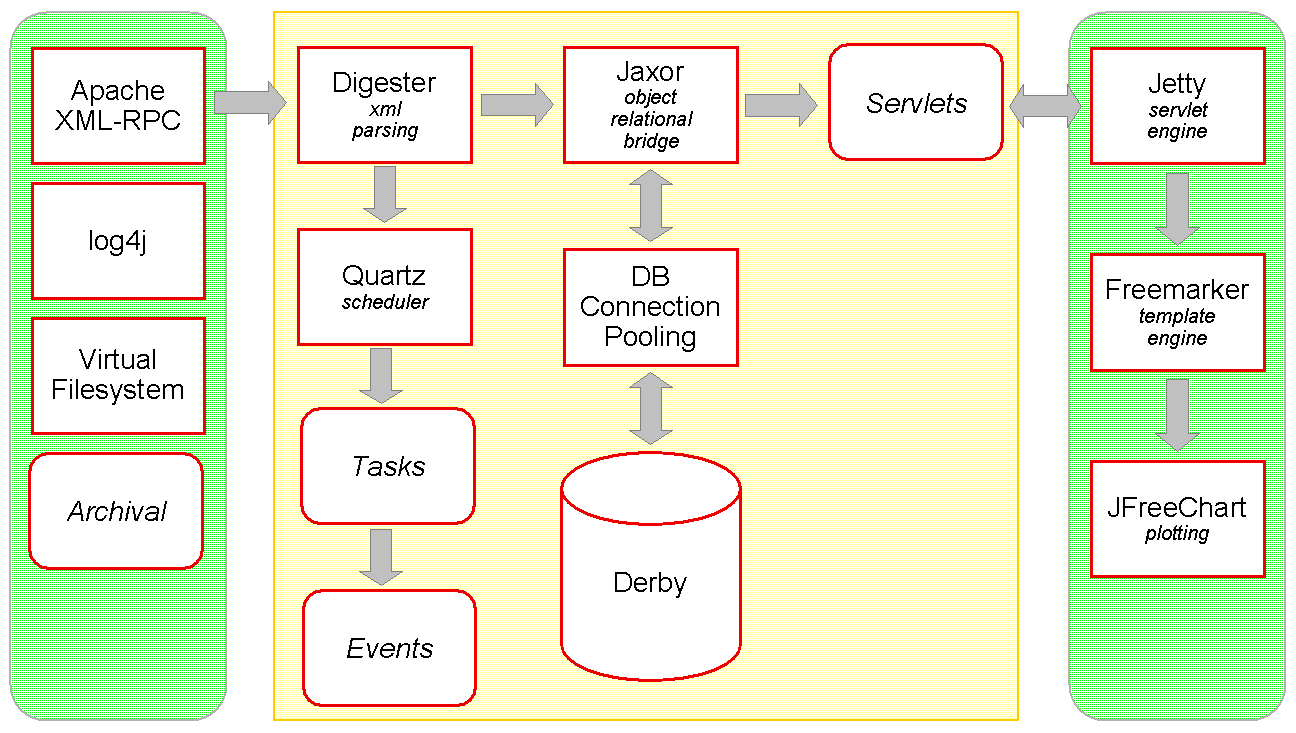
\includegraphics[width=5in]{Dart2-Architecture_v2.png}
	\caption{Dart architecture}
	\label{fig:Dart2-Architecture_v2}
\end{figure}



%----------------------------------------------------------------------
\chapter{Implementation Ideas}
This section captures some implementation ideas.
\section{Server}

\paragraph{Language}
Of all cross-platform languages, Java provides the most robust set of libraries suitable for
Dart.  Java also allows simple distribution of compiled libraries,
\ie jar files, as plug-ins.  Potentially, a client could query
the server for a list of available plug-ins downloading and installing
as needed.

\paragraph{RDBMS}
There are several embeddable Java RDBMS available,
two of the more interesting projects are Cloudscape, recently released
from IBM, and renamed Derby on the Apache site and Hypersonic SQL
(HSQLDB) project hosted on SourceForge.  Dart is envisioned to have a
RDBMS holding summary data; embedding a database into the server
should help to make it transparent and invisible to the casual Dart
user.  For more scalability, the backing store could be any
RDBMS with a JDBC driver.  MySQL and Postgres come to mind.

\paragraph{Transport} 
Though over-designed and complex, SOAP has the elements need to
transmit XML files to the server from the client.  Specifically, SOAP
with attachments could deliver chunks of compressed XML to the server
via HTTP, since most (all?) firewalls allow HTTP traffic. SOAP could
also be used for Dashboard to Dashboard (D2D?)  communication and
remote management and monitoring of Dart servers.  XML-RPC is a much
simpler API, and identically suitable.  XML-RPC will be considered at
the same level as SOAP. Another possible use is dissemination of
plug-ins for clients.  The Java Messaging Service~(JMS) is another
possibility.  JMS gives great flexibility to transport mechanisms and
can operate asynchronously.

\paragraph{Scheduling}
Quartz is an open source enterprise strength
scheduling system for Java.  Quartz will drive scheduled events such
as Dashboard roll ups, DB tasks, and archiving/deletion of old
results.  Quartz will replace cron.

\paragraph{Template Engine}
There are several competing Template engines for Java.  Velocity is an
Apache sponsored project and has some great features including close
integration with other Apache projects.  FreeMarker is another engine
that is more sophisticated than Velocity, but not as integrated.  The
Template engine will be the driver to produce HTML and other reports
replacing XSLT.

\paragraph{Jakarta}  The Apache Jakarta project provides several
packages of immediate use.
\begin{itemize}
\item Digester builds objects from XML,
greatly simplifying configuration from XML files.  Each object is
constructed as needed and automatically configured.
\item CLI should provide a great command line parsing interface.
\item Commons eMail provides a simple java email client.
\item ORO and RegExp, two regular expression packages.
\end{itemize}

\paragraph{Portal}  Though the current Dart HTML pages serve the
purpose well, adding a portal on top would allow custom portlets to be
developed for specific purposes.  For instance, one portlet could be
configured to show a particular build over the last several days, or
perhaps graph the performance of a Test or Result through time across
several architectures.  Dynamic generation of all the Dart results
places undo burden on the server, where a Portal could dynamically
generate limited data in an efficient manner.  One Portal project that
is interesting is Jetspeed 2, an Apache sponsored project.

Portals do add administrative overhead.  It is preferable to
have the ability to use Dart without a Portal, but easily being able
to add the increased utility if desired.


\section{Client}

\chapter{External Packages}
\section{Packages}
Dart is built upon many Open Source packages.  Each of these packages has different licenses.  To comply with the licenses of each of these, we have listed the packages, their licenses and copyrights in this chapter.

\paragraph{Apache v1.1}
Apache XML-RPC, Apache CLI

\paragraph{Apache Version 2.0}
Bean Utilities, Derby, Collections, DBCP, Digester, Pool, VFS, Jetty

\paragraph{BSD License}
Jaxor

\paragraph{Common Public License, v1.0}
JUnit

\paragraph{BSD-Like license}
Quartz 

\paragraph{Freemarker License}
Freemarker

\paragraph{GNU Lesser General Public License}
JFreeChart (http://www.jfree.org/jfreechart/)

\paragraph{HTTPUnit License}
HTTPUnit

\paragraph{CyberNeko Software License, Version 1.0}
NekoHTML


\section{Apache License, Version 1.1}
\begin{verbatim}
The Apache Software License, Version 1.1


Copyright (c) 2001 The Apache Software Foundation.  All rights
reserved.

Redistribution and use in source and binary forms, with or without
modification, are permitted provided that the following conditions
are met:

1. Redistributions of source code must retain the above copyright
   notice, this list of conditions and the following disclaimer.

2. Redistributions in binary form must reproduce the above copyright
   notice, this list of conditions and the following disclaimer in
   the documentation and/or other materials provided with the
   distribution.

3. The end-user documentation included with the redistribution,
   if any, must include the following acknowledgment:
      "This product includes software developed by the
       Apache Software Foundation (http://www.apache.org/)."
   Alternately, this acknowledgment may appear in the software itself,
   if and wherever such third-party acknowledgments normally appear.

4. The names "XML-RPC" and "Apache Software Foundation" must
   not be used to endorse or promote products derived from this
   software without prior written permission. For written
   permission, please contact apache@apache.org.

5. Products derived from this software may not be called "Apache",
   nor may "Apache" appear in their name, without prior written
   permission of the Apache Software Foundation.

THIS SOFTWARE IS PROVIDED ``AS IS'' AND ANY EXPRESSED OR IMPLIED
WARRANTIES, INCLUDING, BUT NOT LIMITED TO, THE IMPLIED WARRANTIES
OF MERCHANTABILITY AND FITNESS FOR A PARTICULAR PURPOSE ARE
DISCLAIMED.  IN NO EVENT SHALL THE APACHE SOFTWARE FOUNDATION OR
ITS CONTRIBUTORS BE LIABLE FOR ANY DIRECT, INDIRECT, INCIDENTAL,
SPECIAL, EXEMPLARY, OR CONSEQUENTIAL DAMAGES (INCLUDING, BUT NOT
LIMITED TO, PROCUREMENT OF SUBSTITUTE GOODS OR SERVICES; LOSS OF
USE, DATA, OR PROFITS; OR BUSINESS INTERRUPTION) HOWEVER CAUSED AND
ON ANY THEORY OF LIABILITY, WHETHER IN CONTRACT, STRICT LIABILITY,
OR TORT (INCLUDING NEGLIGENCE OR OTHERWISE) ARISING IN ANY WAY OUT
OF THE USE OF THIS SOFTWARE, EVEN IF ADVISED OF THE POSSIBILITY OF
SUCH DAMAGE.
====================================================================

This software consists of voluntary contributions made by many
individuals on behalf of the Apache Software Foundation.  For more
information on the Apache Software Foundation, please see
<http://www.apache.org/>.
\end{verbatim}
\section{Apache License, Version 2.0}
\begin{verbatim}

                                 Apache License
                           Version 2.0, January 2004
                        http://www.apache.org/licenses/

   TERMS AND CONDITIONS FOR USE, REPRODUCTION, AND DISTRIBUTION

   1. Definitions.

      "License" shall mean the terms and conditions for use, reproduction,
      and distribution as defined by Sections 1 through 9 of this document.

      "Licensor" shall mean the copyright owner or entity authorized by
      the copyright owner that is granting the License.

      "Legal Entity" shall mean the union of the acting entity and all
      other entities that control, are controlled by, or are under common
      control with that entity. For the purposes of this definition,
      "control" means (i) the power, direct or indirect, to cause the
      direction or management of such entity, whether by contract or
      otherwise, or (ii) ownership of fifty percent (50%) or more of the
      outstanding shares, or (iii) beneficial ownership of such entity.

      "You" (or "Your") shall mean an individual or Legal Entity
      exercising permissions granted by this License.

      "Source" form shall mean the preferred form for making modifications,
      including but not limited to software source code, documentation
      source, and configuration files.

      "Object" form shall mean any form resulting from mechanical
      transformation or translation of a Source form, including but
      not limited to compiled object code, generated documentation,
      and conversions to other media types.

      "Work" shall mean the work of authorship, whether in Source or
      Object form, made available under the License, as indicated by a
      copyright notice that is included in or attached to the work
      (an example is provided in the Appendix below).

      "Derivative Works" shall mean any work, whether in Source or Object
      form, that is based on (or derived from) the Work and for which the
      editorial revisions, annotations, elaborations, or other modifications
      represent, as a whole, an original work of authorship. For the purposes
      of this License, Derivative Works shall not include works that remain
      separable from, or merely link (or bind by name) to the interfaces of,
      the Work and Derivative Works thereof.

      "Contribution" shall mean any work of authorship, including
      the original version of the Work and any modifications or additions
      to that Work or Derivative Works thereof, that is intentionally
      submitted to Licensor for inclusion in the Work by the copyright owner
      or by an individual or Legal Entity authorized to submit on behalf of
      the copyright owner. For the purposes of this definition, "submitted"
      means any form of electronic, verbal, or written communication sent
      to the Licensor or its representatives, including but not limited to
      communication on electronic mailing lists, source code control systems,
      and issue tracking systems that are managed by, or on behalf of, the
      Licensor for the purpose of discussing and improving the Work, but
      excluding communication that is conspicuously marked or otherwise
      designated in writing by the copyright owner as "Not a Contribution."

      "Contributor" shall mean Licensor and any individual or Legal Entity
      on behalf of whom a Contribution has been received by Licensor and
      subsequently incorporated within the Work.

   2. Grant of Copyright License. Subject to the terms and conditions of
      this License, each Contributor hereby grants to You a perpetual,
      worldwide, non-exclusive, no-charge, royalty-free, irrevocable
      copyright license to reproduce, prepare Derivative Works of,
      publicly display, publicly perform, sublicense, and distribute the
      Work and such Derivative Works in Source or Object form.

   3. Grant of Patent License. Subject to the terms and conditions of
      this License, each Contributor hereby grants to You a perpetual,
      worldwide, non-exclusive, no-charge, royalty-free, irrevocable
      (except as stated in this section) patent license to make, have made,
      use, offer to sell, sell, import, and otherwise transfer the Work,
      where such license applies only to those patent claims licensable
      by such Contributor that are necessarily infringed by their
      Contribution(s) alone or by combination of their Contribution(s)
      with the Work to which such Contribution(s) was submitted. If You
      institute patent litigation against any entity (including a
      cross-claim or counterclaim in a lawsuit) alleging that the Work
      or a Contribution incorporated within the Work constitutes direct
      or contributory patent infringement, then any patent licenses
      granted to You under this License for that Work shall terminate
      as of the date such litigation is filed.

   4. Redistribution. You may reproduce and distribute copies of the
      Work or Derivative Works thereof in any medium, with or without
      modifications, and in Source or Object form, provided that You
      meet the following conditions:

      (a) You must give any other recipients of the Work or
          Derivative Works a copy of this License; and

      (b) You must cause any modified files to carry prominent notices
          stating that You changed the files; and

      (c) You must retain, in the Source form of any Derivative Works
          that You distribute, all copyright, patent, trademark, and
          attribution notices from the Source form of the Work,
          excluding those notices that do not pertain to any part of
          the Derivative Works; and

      (d) If the Work includes a "NOTICE" text file as part of its
          distribution, then any Derivative Works that You distribute must
          include a readable copy of the attribution notices contained
          within such NOTICE file, excluding those notices that do not
          pertain to any part of the Derivative Works, in at least one
          of the following places: within a NOTICE text file distributed
          as part of the Derivative Works; within the Source form or
          documentation, if provided along with the Derivative Works; or,
          within a display generated by the Derivative Works, if and
          wherever such third-party notices normally appear. The contents
          of the NOTICE file are for informational purposes only and
          do not modify the License. You may add Your own attribution
          notices within Derivative Works that You distribute, alongside
          or as an addendum to the NOTICE text from the Work, provided
          that such additional attribution notices cannot be construed
          as modifying the License.

      You may add Your own copyright statement to Your modifications and
      may provide additional or different license terms and conditions
      for use, reproduction, or distribution of Your modifications, or
      for any such Derivative Works as a whole, provided Your use,
      reproduction, and distribution of the Work otherwise complies with
      the conditions stated in this License.

   5. Submission of Contributions. Unless You explicitly state otherwise,
      any Contribution intentionally submitted for inclusion in the Work
      by You to the Licensor shall be under the terms and conditions of
      this License, without any additional terms or conditions.
      Notwithstanding the above, nothing herein shall supersede or modify
      the terms of any separate license agreement you may have executed
      with Licensor regarding such Contributions.

   6. Trademarks. This License does not grant permission to use the trade
      names, trademarks, service marks, or product names of the Licensor,
      except as required for reasonable and customary use in describing the
      origin of the Work and reproducing the content of the NOTICE file.

   7. Disclaimer of Warranty. Unless required by applicable law or
      agreed to in writing, Licensor provides the Work (and each
      Contributor provides its Contributions) on an "AS IS" BASIS,
      WITHOUT WARRANTIES OR CONDITIONS OF ANY KIND, either express or
      implied, including, without limitation, any warranties or conditions
      of TITLE, NON-INFRINGEMENT, MERCHANTABILITY, or FITNESS FOR A
      PARTICULAR PURPOSE. You are solely responsible for determining the
      appropriateness of using or redistributing the Work and assume any
      risks associated with Your exercise of permissions under this License.

   8. Limitation of Liability. In no event and under no legal theory,
      whether in tort (including negligence), contract, or otherwise,
      unless required by applicable law (such as deliberate and grossly
      negligent acts) or agreed to in writing, shall any Contributor be
      liable to You for damages, including any direct, indirect, special,
      incidental, or consequential damages of any character arising as a
      result of this License or out of the use or inability to use the
      Work (including but not limited to damages for loss of goodwill,
      work stoppage, computer failure or malfunction, or any and all
      other commercial damages or losses), even if such Contributor
      has been advised of the possibility of such damages.

   9. Accepting Warranty or Additional Liability. While redistributing
      the Work or Derivative Works thereof, You may choose to offer,
      and charge a fee for, acceptance of support, warranty, indemnity,
      or other liability obligations and/or rights consistent with this
      License. However, in accepting such obligations, You may act only
      on Your own behalf and on Your sole responsibility, not on behalf
      of any other Contributor, and only if You agree to indemnify,
      defend, and hold each Contributor harmless for any liability
      incurred by, or claims asserted against, such Contributor by reason
      of your accepting any such warranty or additional liability.

   END OF TERMS AND CONDITIONS

   APPENDIX: How to apply the Apache License to your work.

      To apply the Apache License to your work, attach the following
      boilerplate notice, with the fields enclosed by brackets "[]"
      replaced with your own identifying information. (Don't include
      the brackets!)  The text should be enclosed in the appropriate
      comment syntax for the file format. We also recommend that a
      file or class name and description of purpose be included on the
      same "printed page" as the copyright notice for easier
      identification within third-party archives.

   Copyright [yyyy] [name of copyright owner]

   Licensed under the Apache License, Version 2.0 (the "License");
   you may not use this file except in compliance with the License.
   You may obtain a copy of the License at

       http://www.apache.org/licenses/LICENSE-2.0

   Unless required by applicable law or agreed to in writing, software
   distributed under the License is distributed on an "AS IS" BASIS,
   WITHOUT WARRANTIES OR CONDITIONS OF ANY KIND, either express or implied.
   See the License for the specific language governing permissions and
   limitations under the License.
\end{verbatim}

\section{BSD License}
\begin{verbatim}
Copyright (c) <YEAR>, <OWNER>
All rights reserved.

Redistribution and use in source and binary forms, with or without
modification, are permitted provided that the following conditions are
met:

    * Redistributions of source code must retain the above copyright
    * notice, this list of conditions and the following disclaimer.

    * Redistributions in binary form must reproduce the above
    * copyright notice, this list of conditions and the following
    * disclaimer in the documentation and/or other materials provided
    * with the distribution.

    * Neither the name of the <ORGANIZATION> nor the names of its
    * contributors may be used to endorse or promote products derived
    * from this software without specific prior written permission.

THIS SOFTWARE IS PROVIDED BY THE COPYRIGHT HOLDERS AND CONTRIBUTORS
"AS IS" AND ANY EXPRESS OR IMPLIED WARRANTIES, INCLUDING, BUT NOT
LIMITED TO, THE IMPLIED WARRANTIES OF MERCHANTABILITY AND FITNESS FOR
A PARTICULAR PURPOSE ARE DISCLAIMED. IN NO EVENT SHALL THE COPYRIGHT
OWNER OR CONTRIBUTORS BE LIABLE FOR ANY DIRECT, INDIRECT, INCIDENTAL,
SPECIAL, EXEMPLARY, OR CONSEQUENTIAL DAMAGES (INCLUDING, BUT NOT
LIMITED TO, PROCUREMENT OF SUBSTITUTE GOODS OR SERVICES; LOSS OF USE,
DATA, OR PROFITS; OR BUSINESS INTERRUPTION) HOWEVER CAUSED AND ON ANY
THEORY OF LIABILITY, WHETHER IN CONTRACT, STRICT LIABILITY, OR TORT
(INCLUDING NEGLIGENCE OR OTHERWISE) ARISING IN ANY WAY OUT OF THE USE
OF THIS SOFTWARE, EVEN IF ADVISED OF THE POSSIBILITY OF SUCH DAMAGE.

\end{verbatim}

\section{Freemarker License}
\begin{verbatim}
Copyright (c) 2003 The Visigoth Software Society. All rights reserved.

Redistribution and use in source and binary forms, with or without
modification, are permitted provided that the following conditions are met:

1.  Redistributions of source code must retain the above copyright notice,
    this list of conditions and the following disclaimer.

2.  The end-user documentation included with the redistribution, if any, must
    include the following acknowledgment:
      "This product includes software developed by the 
      Visigoth Software Society (http://www.visigoths.org/)."
    Alternately, this acknowledgment may appear in the software itself, if and
    wherever such third-party acknowledgments normally appear.

3.  Neither the name "FreeMarker", "Visigoth", nor any of the names of the
    project contributors may be used to endorse or promote products derived
    from this software without prior written permission. For written
    permission, please contact visigoths@visigoths.org.

4.  Products derived from this software may not be called "FreeMarker" or
    "Visigoth" nor may "FreeMarker" or "Visigoth" appear in their names
    without prior written permission of the Visigoth Software Society.

THIS SOFTWARE IS PROVIDED ``AS IS'' AND ANY EXPRESSED OR IMPLIED WARRANTIES,
INCLUDING, BUT NOT LIMITED TO, THE IMPLIED WARRANTIES OF MERCHANTABILITY AND
FITNESS FOR A PARTICULAR PURPOSE ARE DISCLAIMED. IN NO EVENT SHALL THE
VISIGOTH SOFTWARE SOCIETY OR ITS CONTRIBUTORS BE LIABLE FOR ANY DIRECT,
INDIRECT, INCIDENTAL, SPECIAL, EXEMPLARY, OR CONSEQUENTIAL DAMAGES (INCLUDING,
BUT NOT LIMITED TO, PROCUREMENT OF SUBSTITUTE GOODS OR SERVICES; LOSS OF USE,
DATA, OR PROFITS; OR BUSINESS INTERRUPTION) HOWEVER CAUSED AND ON ANY THEORY
OF LIABILITY, WHETHER IN CONTRACT, STRICT LIABILITY, OR TORT (INCLUDING
NEGLIGENCE OR OTHERWISE) ARISING IN ANY WAY OUT OF THE USE OF THIS SOFTWARE,
EVEN IF ADVISED OF THE POSSIBILITY OF SUCH DAMAGE.
\end{verbatim}

\section{Quartz License}
\begin{verbatim}
 Copyright James House (c) 2001-2004

 All rights reserved.

Redistribution and use in source and binary forms, with or without
modification, are permitted provided that the following conditions
are met:
1. Redistributions of source code must retain the above copyright
   notice, this list of conditions and the following disclaimer.
2. Redistributions in binary form must reproduce the above copyright
   notice, this list of conditions and the following disclaimer in the
   documentation and/or other materials provided with the distribution.

THIS SOFTWARE IS PROVIDED BY THE AUTHOR AND CONTRIBUTORS ``AS IS'' AND
ANY EXPRESS OR IMPLIED WARRANTIES, INCLUDING, BUT NOT LIMITED TO, THE
IMPLIED WARRANTIES OF MERCHANTABILITY AND FITNESS FOR A PARTICULAR PURPOSE
ARE DISCLAIMED.  IN NO EVENT SHALL THE AUTHOR OR CONTRIBUTORS BE LIABLE
FOR ANY DIRECT, INDIRECT, INCIDENTAL, SPECIAL, EXEMPLARY, OR CONSEQUENTIAL
DAMAGES (INCLUDING, BUT NOT LIMITED TO, PROCUREMENT OF SUBSTITUTE GOODS
OR SERVICES; LOSS OF USE, DATA, OR PROFITS; OR BUSINESS INTERRUPTION)
HOWEVER CAUSED AND ON ANY THEORY OF LIABILITY, WHETHER IN CONTRACT, STRICT
LIABILITY, OR TORT (INCLUDING NEGLIGENCE OR OTHERWISE) ARISING IN ANY WAY
OUT OF THE USE OF THIS SOFTWARE, EVEN IF ADVISED OF THE POSSIBILITY OF
SUCH DAMAGE.
\end{verbatim}

                
\section{GNU Lesser General Public License}
\begin{verbatim}
                  GNU LESSER GENERAL PUBLIC LICENSE
                       Version 2.1, February 1999

 Copyright (C) 1991, 1999 Free Software Foundation, Inc.
     59 Temple Place, Suite 330, Boston, MA  02111-1307  USA
 Everyone is permitted to copy and distribute verbatim copies
 of this license document, but changing it is not allowed.

[This is the first released version of the Lesser GPL.  It also counts
 as the successor of the GNU Library Public License, version 2, hence
 the version number 2.1.]

                            Preamble

  The licenses for most software are designed to take away your
freedom to share and change it.  By contrast, the GNU General Public
Licenses are intended to guarantee your freedom to share and change
free software--to make sure the software is free for all its users.

  This license, the Lesser General Public License, applies to some
specially designated software packages--typically libraries--of the
Free Software Foundation and other authors who decide to use it.  You
can use it too, but we suggest you first think carefully about whether
this license or the ordinary General Public License is the better
strategy to use in any particular case, based on the explanations below.

  When we speak of free software, we are referring to freedom of use,
not price.  Our General Public Licenses are designed to make sure that
you have the freedom to distribute copies of free software (and charge
for this service if you wish); that you receive source code or can get
it if you want it; that you can change the software and use pieces of
it in new free programs; and that you are informed that you can do
these things.

  To protect your rights, we need to make restrictions that forbid
distributors to deny you these rights or to ask you to surrender these
rights.  These restrictions translate to certain responsibilities for
you if you distribute copies of the library or if you modify it.

  For example, if you distribute copies of the library, whether gratis
or for a fee, you must give the recipients all the rights that we gave
you.  You must make sure that they, too, receive or can get the source
code.  If you link other code with the library, you must provide
complete object files to the recipients, so that they can relink them
with the library after making changes to the library and recompiling
it.  And you must show them these terms so they know their rights.

  We protect your rights with a two-step method: (1) we copyright the
library, and (2) we offer you this license, which gives you legal
permission to copy, distribute and/or modify the library.

  To protect each distributor, we want to make it very clear that
there is no warranty for the free library.  Also, if the library is
modified by someone else and passed on, the recipients should know
that what they have is not the original version, so that the original
author's reputation will not be affected by problems that might be
introduced by others.

  Finally, software patents pose a constant threat to the existence of
any free program.  We wish to make sure that a company cannot
effectively restrict the users of a free program by obtaining a
restrictive license from a patent holder.  Therefore, we insist that
any patent license obtained for a version of the library must be
consistent with the full freedom of use specified in this license.

  Most GNU software, including some libraries, is covered by the
ordinary GNU General Public License.  This license, the GNU Lesser
General Public License, applies to certain designated libraries, and
is quite different from the ordinary General Public License.  We use
this license for certain libraries in order to permit linking those
libraries into non-free programs.

  When a program is linked with a library, whether statically or using
a shared library, the combination of the two is legally speaking a
combined work, a derivative of the original library.  The ordinary
General Public License therefore permits such linking only if the
entire combination fits its criteria of freedom.  The Lesser General
Public License permits more lax criteria for linking other code with
the library.

  We call this license the "Lesser" General Public License because it
does Less to protect the user's freedom than the ordinary General
Public License.  It also provides other free software developers Less
of an advantage over competing non-free programs.  These disadvantages
are the reason we use the ordinary General Public License for many
libraries.  However, the Lesser license provides advantages in certain
special circumstances.

  For example, on rare occasions, there may be a special need to
encourage the widest possible use of a certain library, so that it becomes
a de-facto standard.  To achieve this, non-free programs must be
allowed to use the library.  A more frequent case is that a free
library does the same job as widely used non-free libraries.  In this
case, there is little to gain by limiting the free library to free
software only, so we use the Lesser General Public License.

  In other cases, permission to use a particular library in non-free
programs enables a greater number of people to use a large body of
free software.  For example, permission to use the GNU C Library in
non-free programs enables many more people to use the whole GNU
operating system, as well as its variant, the GNU/Linux operating
system.

  Although the Lesser General Public License is Less protective of the
users' freedom, it does ensure that the user of a program that is
linked with the Library has the freedom and the wherewithal to run
that program using a modified version of the Library.

  The precise terms and conditions for copying, distribution and
modification follow.  Pay close attention to the difference between a
"work based on the library" and a "work that uses the library".  The
former contains code derived from the library, whereas the latter must
be combined with the library in order to run.

                  GNU LESSER GENERAL PUBLIC LICENSE
   TERMS AND CONDITIONS FOR COPYING, DISTRIBUTION AND MODIFICATION

  0. This License Agreement applies to any software library or other
program which contains a notice placed by the copyright holder or
other authorized party saying it may be distributed under the terms of
this Lesser General Public License (also called "this License").
Each licensee is addressed as "you".

  A "library" means a collection of software functions and/or data
prepared so as to be conveniently linked with application programs
(which use some of those functions and data) to form executables.

  The "Library", below, refers to any such software library or work
which has been distributed under these terms.  A "work based on the
Library" means either the Library or any derivative work under
copyright law: that is to say, a work containing the Library or a
portion of it, either verbatim or with modifications and/or translated
straightforwardly into another language.  (Hereinafter, translation is
included without limitation in the term "modification".)

  "Source code" for a work means the preferred form of the work for
making modifications to it.  For a library, complete source code means
all the source code for all modules it contains, plus any associated
interface definition files, plus the scripts used to control compilation
and installation of the library.

  Activities other than copying, distribution and modification are not
covered by this License; they are outside its scope.  The act of
running a program using the Library is not restricted, and output from
such a program is covered only if its contents constitute a work based
on the Library (independent of the use of the Library in a tool for
writing it).  Whether that is true depends on what the Library does
and what the program that uses the Library does.
  
  1. You may copy and distribute verbatim copies of the Library's
complete source code as you receive it, in any medium, provided that
you conspicuously and appropriately publish on each copy an
appropriate copyright notice and disclaimer of warranty; keep intact
all the notices that refer to this License and to the absence of any
warranty; and distribute a copy of this License along with the
Library.

  You may charge a fee for the physical act of transferring a copy,
and you may at your option offer warranty protection in exchange for a
fee.

  2. You may modify your copy or copies of the Library or any portion
of it, thus forming a work based on the Library, and copy and
distribute such modifications or work under the terms of Section 1
above, provided that you also meet all of these conditions:

    a) The modified work must itself be a software library.

    b) You must cause the files modified to carry prominent notices
    stating that you changed the files and the date of any change.

    c) You must cause the whole of the work to be licensed at no
    charge to all third parties under the terms of this License.

    d) If a facility in the modified Library refers to a function or a
    table of data to be supplied by an application program that uses
    the facility, other than as an argument passed when the facility
    is invoked, then you must make a good faith effort to ensure that,
    in the event an application does not supply such function or
    table, the facility still operates, and performs whatever part of
    its purpose remains meaningful.

    (For example, a function in a library to compute square roots has
    a purpose that is entirely well-defined independent of the
    application.  Therefore, Subsection 2d requires that any
    application-supplied function or table used by this function must
    be optional: if the application does not supply it, the square
    root function must still compute square roots.)

These requirements apply to the modified work as a whole.  If
identifiable sections of that work are not derived from the Library,
and can be reasonably considered independent and separate works in
themselves, then this License, and its terms, do not apply to those
sections when you distribute them as separate works.  But when you
distribute the same sections as part of a whole which is a work based
on the Library, the distribution of the whole must be on the terms of
this License, whose permissions for other licensees extend to the
entire whole, and thus to each and every part regardless of who wrote
it.

Thus, it is not the intent of this section to claim rights or contest
your rights to work written entirely by you; rather, the intent is to
exercise the right to control the distribution of derivative or
collective works based on the Library.

In addition, mere aggregation of another work not based on the Library
with the Library (or with a work based on the Library) on a volume of
a storage or distribution medium does not bring the other work under
the scope of this License.

  3. You may opt to apply the terms of the ordinary GNU General Public
License instead of this License to a given copy of the Library.  To do
this, you must alter all the notices that refer to this License, so
that they refer to the ordinary GNU General Public License, version 2,
instead of to this License.  (If a newer version than version 2 of the
ordinary GNU General Public License has appeared, then you can specify
that version instead if you wish.)  Do not make any other change in
these notices.

  Once this change is made in a given copy, it is irreversible for
that copy, so the ordinary GNU General Public License applies to all
subsequent copies and derivative works made from that copy.

  This option is useful when you wish to copy part of the code of
the Library into a program that is not a library.

  4. You may copy and distribute the Library (or a portion or
derivative of it, under Section 2) in object code or executable form
under the terms of Sections 1 and 2 above provided that you accompany
it with the complete corresponding machine-readable source code, which
must be distributed under the terms of Sections 1 and 2 above on a
medium customarily used for software interchange.

  If distribution of object code is made by offering access to copy
from a designated place, then offering equivalent access to copy the
source code from the same place satisfies the requirement to
distribute the source code, even though third parties are not
compelled to copy the source along with the object code.

  5. A program that contains no derivative of any portion of the
Library, but is designed to work with the Library by being compiled or
linked with it, is called a "work that uses the Library".  Such a
work, in isolation, is not a derivative work of the Library, and
therefore falls outside the scope of this License.

  However, linking a "work that uses the Library" with the Library
creates an executable that is a derivative of the Library (because it
contains portions of the Library), rather than a "work that uses the
library".  The executable is therefore covered by this License.
Section 6 states terms for distribution of such executables.

  When a "work that uses the Library" uses material from a header file
that is part of the Library, the object code for the work may be a
derivative work of the Library even though the source code is not.
Whether this is true is especially significant if the work can be
linked without the Library, or if the work is itself a library.  The
threshold for this to be true is not precisely defined by law.

  If such an object file uses only numerical parameters, data
structure layouts and accessors, and small macros and small inline
functions (ten lines or less in length), then the use of the object
file is unrestricted, regardless of whether it is legally a derivative
work.  (Executables containing this object code plus portions of the
Library will still fall under Section 6.)

  Otherwise, if the work is a derivative of the Library, you may
distribute the object code for the work under the terms of Section 6.
Any executables containing that work also fall under Section 6,
whether or not they are linked directly with the Library itself.

  6. As an exception to the Sections above, you may also combine or
link a "work that uses the Library" with the Library to produce a
work containing portions of the Library, and distribute that work
under terms of your choice, provided that the terms permit
modification of the work for the customer's own use and reverse
engineering for debugging such modifications.

  You must give prominent notice with each copy of the work that the
Library is used in it and that the Library and its use are covered by
this License.  You must supply a copy of this License.  If the work
during execution displays copyright notices, you must include the
copyright notice for the Library among them, as well as a reference
directing the user to the copy of this License.  Also, you must do one
of these things:

    a) Accompany the work with the complete corresponding
    machine-readable source code for the Library including whatever
    changes were used in the work (which must be distributed under
    Sections 1 and 2 above); and, if the work is an executable linked
    with the Library, with the complete machine-readable "work that
    uses the Library", as object code and/or source code, so that the
    user can modify the Library and then relink to produce a modified
    executable containing the modified Library.  (It is understood
    that the user who changes the contents of definitions files in the
    Library will not necessarily be able to recompile the application
    to use the modified definitions.)

    b) Use a suitable shared library mechanism for linking with the
    Library.  A suitable mechanism is one that (1) uses at run time a
    copy of the library already present on the user's computer system,
    rather than copying library functions into the executable, and (2)
    will operate properly with a modified version of the library, if
    the user installs one, as long as the modified version is
    interface-compatible with the version that the work was made with.

    c) Accompany the work with a written offer, valid for at
    least three years, to give the same user the materials
    specified in Subsection 6a, above, for a charge no more
    than the cost of performing this distribution.

    d) If distribution of the work is made by offering access to copy
    from a designated place, offer equivalent access to copy the above
    specified materials from the same place.

    e) Verify that the user has already received a copy of these
    materials or that you have already sent this user a copy.

  For an executable, the required form of the "work that uses the
Library" must include any data and utility programs needed for
reproducing the executable from it.  However, as a special exception,
the materials to be distributed need not include anything that is
normally distributed (in either source or binary form) with the major
components (compiler, kernel, and so on) of the operating system on
which the executable runs, unless that component itself accompanies
the executable.

  It may happen that this requirement contradicts the license
restrictions of other proprietary libraries that do not normally
accompany the operating system.  Such a contradiction means you cannot
use both them and the Library together in an executable that you
distribute.

  7. You may place library facilities that are a work based on the
Library side-by-side in a single library together with other library
facilities not covered by this License, and distribute such a combined
library, provided that the separate distribution of the work based on
the Library and of the other library facilities is otherwise
permitted, and provided that you do these two things:

    a) Accompany the combined library with a copy of the same work
    based on the Library, uncombined with any other library
    facilities.  This must be distributed under the terms of the
    Sections above.

    b) Give prominent notice with the combined library of the fact
    that part of it is a work based on the Library, and explaining
    where to find the accompanying uncombined form of the same work.

  8. You may not copy, modify, sublicense, link with, or distribute
the Library except as expressly provided under this License.  Any
attempt otherwise to copy, modify, sublicense, link with, or
distribute the Library is void, and will automatically terminate your
rights under this License.  However, parties who have received copies,
or rights, from you under this License will not have their licenses
terminated so long as such parties remain in full compliance.

  9. You are not required to accept this License, since you have not
signed it.  However, nothing else grants you permission to modify or
distribute the Library or its derivative works.  These actions are
prohibited by law if you do not accept this License.  Therefore, by
modifying or distributing the Library (or any work based on the
Library), you indicate your acceptance of this License to do so, and
all its terms and conditions for copying, distributing or modifying
the Library or works based on it.

  10. Each time you redistribute the Library (or any work based on the
Library), the recipient automatically receives a license from the
original licensor to copy, distribute, link with or modify the Library
subject to these terms and conditions.  You may not impose any further
restrictions on the recipients' exercise of the rights granted herein.
You are not responsible for enforcing compliance by third parties with
this License.

  11. If, as a consequence of a court judgment or allegation of patent
infringement or for any other reason (not limited to patent issues),
conditions are imposed on you (whether by court order, agreement or
otherwise) that contradict the conditions of this License, they do not
excuse you from the conditions of this License.  If you cannot
distribute so as to satisfy simultaneously your obligations under this
License and any other pertinent obligations, then as a consequence you
may not distribute the Library at all.  For example, if a patent
license would not permit royalty-free redistribution of the Library by
all those who receive copies directly or indirectly through you, then
the only way you could satisfy both it and this License would be to
refrain entirely from distribution of the Library.

If any portion of this section is held invalid or unenforceable under any
particular circumstance, the balance of the section is intended to apply,
and the section as a whole is intended to apply in other circumstances.

It is not the purpose of this section to induce you to infringe any
patents or other property right claims or to contest validity of any
such claims; this section has the sole purpose of protecting the
integrity of the free software distribution system which is
implemented by public license practices.  Many people have made
generous contributions to the wide range of software distributed
through that system in reliance on consistent application of that
system; it is up to the author/donor to decide if he or she is willing
to distribute software through any other system and a licensee cannot
impose that choice.

This section is intended to make thoroughly clear what is believed to
be a consequence of the rest of this License.

  12. If the distribution and/or use of the Library is restricted in
certain countries either by patents or by copyrighted interfaces, the
original copyright holder who places the Library under this License may add
an explicit geographical distribution limitation excluding those countries,
so that distribution is permitted only in or among countries not thus
excluded.  In such case, this License incorporates the limitation as if
written in the body of this License.

  13. The Free Software Foundation may publish revised and/or new
versions of the Lesser General Public License from time to time.
Such new versions will be similar in spirit to the present version,
but may differ in detail to address new problems or concerns.

Each version is given a distinguishing version number.  If the Library
specifies a version number of this License which applies to it and
"any later version", you have the option of following the terms and
conditions either of that version or of any later version published by
the Free Software Foundation.  If the Library does not specify a
license version number, you may choose any version ever published by
the Free Software Foundation.

  14. If you wish to incorporate parts of the Library into other free
programs whose distribution conditions are incompatible with these,
write to the author to ask for permission.  For software which is
copyrighted by the Free Software Foundation, write to the Free
Software Foundation; we sometimes make exceptions for this.  Our
decision will be guided by the two goals of preserving the free status
of all derivatives of our free software and of promoting the sharing
and reuse of software generally.

                            NO WARRANTY

  15. BECAUSE THE LIBRARY IS LICENSED FREE OF CHARGE, THERE IS NO
WARRANTY FOR THE LIBRARY, TO THE EXTENT PERMITTED BY APPLICABLE LAW.
EXCEPT WHEN OTHERWISE STATED IN WRITING THE COPYRIGHT HOLDERS AND/OR
OTHER PARTIES PROVIDE THE LIBRARY "AS IS" WITHOUT WARRANTY OF ANY
KIND, EITHER EXPRESSED OR IMPLIED, INCLUDING, BUT NOT LIMITED TO, THE
IMPLIED WARRANTIES OF MERCHANTABILITY AND FITNESS FOR A PARTICULAR
PURPOSE.  THE ENTIRE RISK AS TO THE QUALITY AND PERFORMANCE OF THE
LIBRARY IS WITH YOU.  SHOULD THE LIBRARY PROVE DEFECTIVE, YOU ASSUME
THE COST OF ALL NECESSARY SERVICING, REPAIR OR CORRECTION.

  16. IN NO EVENT UNLESS REQUIRED BY APPLICABLE LAW OR AGREED TO IN
WRITING WILL ANY COPYRIGHT HOLDER, OR ANY OTHER PARTY WHO MAY MODIFY
AND/OR REDISTRIBUTE THE LIBRARY AS PERMITTED ABOVE, BE LIABLE TO YOU
FOR DAMAGES, INCLUDING ANY GENERAL, SPECIAL, INCIDENTAL OR
CONSEQUENTIAL DAMAGES ARISING OUT OF THE USE OR INABILITY TO USE THE
LIBRARY (INCLUDING BUT NOT LIMITED TO LOSS OF DATA OR DATA BEING
RENDERED INACCURATE OR LOSSES SUSTAINED BY YOU OR THIRD PARTIES OR A
FAILURE OF THE LIBRARY TO OPERATE WITH ANY OTHER SOFTWARE), EVEN IF
SUCH HOLDER OR OTHER PARTY HAS BEEN ADVISED OF THE POSSIBILITY OF SUCH
DAMAGES.

                     END OF TERMS AND CONDITIONS

           How to Apply These Terms to Your New Libraries

  If you develop a new library, and you want it to be of the greatest
possible use to the public, we recommend making it free software that
everyone can redistribute and change.  You can do so by permitting
redistribution under these terms (or, alternatively, under the terms of the
ordinary General Public License).

  To apply these terms, attach the following notices to the library.  It is
safest to attach them to the start of each source file to most effectively
convey the exclusion of warranty; and each file should have at least the
"copyright" line and a pointer to where the full notice is found.

    <one line to give the library's name and a brief idea of what it does.>
    Copyright (C) <year>  <name of author>

    This library is free software; you can redistribute it and/or
    modify it under the terms of the GNU Lesser General Public
    License as published by the Free Software Foundation; either
    version 2.1 of the License, or (at your option) any later version.

    This library is distributed in the hope that it will be useful,
    but WITHOUT ANY WARRANTY; without even the implied warranty of
    MERCHANTABILITY or FITNESS FOR A PARTICULAR PURPOSE.  See the GNU
    Lesser General Public License for more details.

    You should have received a copy of the GNU Lesser General Public
    License along with this library; if not, write to the Free Software
    Foundation, Inc., 59 Temple Place, Suite 330, Boston, MA  02111-1307  USA

Also add information on how to contact you by electronic and paper mail.

You should also get your employer (if you work as a programmer) or your
school, if any, to sign a "copyright disclaimer" for the library, if
necessary.  Here is a sample; alter the names:

  Yoyodyne, Inc., hereby disclaims all copyright interest in the
  library `Frob' (a library for tweaking knobs) written by James Random Hacker.

  <signature of Ty Coon>, 1 April 1990
  Ty Coon, President of Vice

That's all there is to it!
\end{verbatim}


\section{HTTPUnit license}

\begin{verbatim}
Copyright � 2000-2004, Russell Gold

Permission is hereby granted, free of charge, to any person obtaining
a copy of this software and associated documentation files (the
"Software"), to deal in the Software without restriction, including
without limitation the rights to use, copy, modify, merge, publish,
distribute, sublicense, and/or sell copies of the Software, and to
permit persons to whom the Software is furnished to do so, subject to
the following conditions:

The above copyright notice and this permission notice shall be
included in all copies or substantial portions of the Software.

THE SOFTWARE IS PROVIDED "AS IS", WITHOUT WARRANTY OF ANY KIND,
EXPRESS OR IMPLIED, INCLUDING BUT NOT LIMITED TO THE WARRANTIES OF
MERCHANTABILITY, FITNESS FOR A PARTICULAR PURPOSE AND NONINFRINGEMENT.
IN NO EVENT SHALL THE AUTHORS OR COPYRIGHT HOLDERS BE LIABLE FOR ANY
CLAIM, DAMAGES OR OTHER LIABILITY, WHETHER IN AN ACTION OF CONTRACT,
TORT OR OTHERWISE, ARISING FROM, OUT OF OR IN CONNECTION WITH THE
SOFTWARE OR THE USE OR OTHER DEALINGS IN THE SOFTWARE.
\end{verbatim}


\section{CyberNeko Software License}

\begin{verbatim}
The CyberNeko Software License, Version 1.0

 
(C) Copyright 2002-2005, Andy Clark.  All rights reserved.
 
Redistribution and use in source and binary forms, with or without
modification, are permitted provided that the following conditions
are met:

1. Redistributions of source code must retain the above copyright
   notice, this list of conditions and the following disclaimer. 

2. Redistributions in binary form must reproduce the above copyright
   notice, this list of conditions and the following disclaimer in
   the documentation and/or other materials provided with the
   distribution.

3. The end-user documentation included with the redistribution,
   if any, must include the following acknowledgment:  
     "This product includes software developed by Andy Clark."
   Alternately, this acknowledgment may appear in the software itself,
   if and wherever such third-party acknowledgments normally appear.

4. The names "CyberNeko" and "NekoHTML" must not be used to endorse
   or promote products derived from this software without prior 
   written permission. For written permission, please contact 
   andyc@cyberneko.net.

5. Products derived from this software may not be called "CyberNeko",
   nor may "CyberNeko" appear in their name, without prior written
   permission of the author.

THIS SOFTWARE IS PROVIDED ``AS IS'' AND ANY EXPRESSED OR IMPLIED
WARRANTIES, INCLUDING, BUT NOT LIMITED TO, THE IMPLIED WARRANTIES
OF MERCHANTABILITY AND FITNESS FOR A PARTICULAR PURPOSE ARE
DISCLAIMED.  IN NO EVENT SHALL THE AUTHOR OR OTHER CONTRIBUTORS
BE LIABLE FOR ANY DIRECT, INDIRECT, INCIDENTAL, SPECIAL, EXEMPLARY, 
OR CONSEQUENTIAL DAMAGES (INCLUDING, BUT NOT LIMITED TO, PROCUREMENT 
OF SUBSTITUTE GOODS OR SERVICES; LOSS OF USE, DATA, OR PROFITS; OR 
BUSINESS INTERRUPTION) HOWEVER CAUSED AND ON ANY THEORY OF LIABILITY, 
WHETHER IN CONTRACT, STRICT LIABILITY, OR TORT (INCLUDING NEGLIGENCE 
OR OTHERWISE) ARISING IN ANY WAY OUT OF THE USE OF THIS SOFTWARE, 
EVEN IF ADVISED OF THE POSSIBILITY OF SUCH DAMAGE.

====================================================================

This license is based on the Apache Software License, version 1.1.
\end{verbatim}

\end{document}
% LocalWords:  FreeMarker CommandServlet MaxTasks commandline TestServer cron
% LocalWords:  DartServer refreshServer TestProject getstatus logconfiguration
% LocalWords:  getInitParameter CommandManager ChartServlet TaskQueue
% LocalWords:  CronTrigger ListenerManager QueueManager MyDashboard classpath
% LocalWords:  servlet ListenTo xml SaveStatistics ArchiveTask QueueManagerTask
% LocalWords:  GarbageCollectionTask datetime
